\documentclass[10pt, a4paper, twoside]{basestyle}

\usepackage[Mathematics]{semtex}
\usepackage{chngcntr}

\counterwithout{equation}{section}
\renewcommand{\thesubsection}{\arabic{subsection}}

\setcounter{MaxMatrixCols}{20}

% TODO(egg): move to semtex.
\newlength{\medianToZeroTop}
\newcommand\zeroBL[1]{\multicolumn{1}{l}{\rlap{\smash{\text{{#1$0$}}}}}}
\newcommand\zeroBR[1]{\multicolumn{1}{r}{\llap{\smash{\text{{#1$0$}}}}}}
\newcommand\zeroTR[1]{\multicolumn{1}{r}{\llap{\smash{\setlength{\medianToZeroTop}{\heightof{#1$0$}-1ex}\raisebox{-\medianToZeroTop}{\text{{#1$0$}}}}}}}

% TODO(egg): move to basestyle.
\usepackage[all]{nowidow}
\usepackage{tabls}
\usepackage{changepage}
\usepackage[xetex,outerbars]{changebar}

%%%% Shorthands.
\DeclareMathOperator{\bias}{\mathit{bias}}
% Rounding brackets will be heavily nested, and reading the nesting depth is critically important,
% so we make them grow for readability.
\newcommand{\round}[1]{\doubleSquareBrackets*{#1}}
\newcommand{\roundTowardZero}[1]{\doubleSquareBrackets{#1}_0}
\newcommand{\roundTowardPositive}[1]{\doubleSquareBrackets{#1}_+}
\newcommand{\roundTowardNegative}[1]{\doubleSquareBrackets{#1}_-}
\newcommand{\hex}[1]{{_{16}}\mathrm{#1}}
\newcommand{\bin}[1]{{_{2}}\mathrm{#1}}

% For alignment of tabular rounding error analyses.
\DeclareDelimiter\doubleSquareBracketEmptyUnkerned{\lBrack}{.}
\newcommand{\leftRound}[1]{\doubleSquareBracketEmptyUnkerned*{#1\kern-\nulldelimiterspace}}

\newcommand{\bigradient}[4]{\det\begin{pmatrix}\pa{#1}_{#2}\\\pa{#3}_{#4}\end{pmatrix}}

%%%% Title and authors.

\title{A correctly rounded binary64 cube root}
\date{REMOVE BEFORE FLIGHT \printdate{2021-04-36}}
\author{Robin~Leroy (eggrobin)}
\begin{document}
\maketitle
\noindent
This document describes the implementation of correctly-rounded binary64 cube root function {\texttt{principia::numerics::Cbrt}}
defined in \href{https://github.com/mockingbirdnest/Principia/blob/master/numerics/cbrt.cpp}{\texttt{numerics/cbrt.cpp}}.

\part*{Outline}

Our computation of the cube root uses root-finding methods that have fallen into disuse, and thus may be unfamiliar to the reader.

\cbstart{}To avoid\cbend{} confusion on the properties and names of these methods, this document comprises two parts.
The first one is about a family of root-finding methods for arbitrary functions, wherein all methods
considered for the cube root can be found. The second is about the computation of a binary64 cube root and its error
analysis.

The methods considered in the first part originate from a series of works by Thomas Fantet de~Lagny\footnote{Thomas Fantet de~Lagny (1660--1734), professor
of hydrography in Rochefort, 1697--1714, subdirector then director of Law's \foreign{\textfrench{Banque générale}}.
Member of the \foreign{\textfrench{Académie Royale des Sciences}}. See \cite{Fontenelle1734}, reprinted in \volcite{6}[557\psqq]{Fontenelle1758}.}. Lagny's methods
may be used to find a root of any polynomial; curiously, they are of convergence order $p$ for polynomials of degree $p$.
We give a generalization of these methods which applies to arbitrary functions (and in particular to polynomials
of degree other than the order).

Throughout the centuries, some of Lagny's methods have been rediscovered, whether from Lagny's works or from first principles,
and generalized to arbitrary functions. The reader may be familiar with these special cases, as some of them have remained in
use, and are found in more modern literature; most famous of these is perhaps Halley's (rational) method. We thus show that
these are indeed special cases of the generalization of Lagny's method, and describe the names we use for specific cases,
depending on the order of their discovery.

Our path through more than three centuries of literature to rediscovering---and then generalizing---Lagny's methods led us to
many remarkable works; we mention those in a bibliographic note.

The second part starts with the treatment of a faithfully rounded---and very nearly correctly rounded---cube root.
For each step in the computation of the cube root, we consider multiple alternatives, each with its error analysis; the one that
should be chosen is revealed by the final error analysis.

We then describe how correct rounding is achieved, by determining whether the faithful result might be misrounded,
in which case the correct digit needs to be more carefully ascertained.

In order not to interrupt the flow of reading, in both parts, we relegate to the appendices
any miscellaneous considerations that are independent of the matter currently being discussed,
long-winded proofs, and lists of examples.
\pagebreak



\part{Abridged root-finding methods}
\label{Abridged}
We recall and generalize a family of root-finding methods from the late 17th century.

In \cite{FantetdeLagny1691a}, Lagny first presents the following iterations for the computation of the cube root
$\cuberoot{a^3+b}$:\begin{align}
\FunctionBody*{a}{\tfrac{1}{2}a+\sqrt{\tfrac{1}{4}a^2+\frac{b}{3a}}}\text, \label{LagnyIrrationalCubeRootIteration}
\intertext{hereafter the \emph{(quadratic) irrational method}, and}
\FunctionBody*{a}{a+\frac{ab}{3a^3+b}}\text, \label{LagnyRationalCubeRootIteration}
\end{align}
the \emph{rational method}, mentioning the existence of similar methods for higher powers.
In \cite{FantetdeLagny1691b} the above methods are again given, with an outline
of the general method for higher powers, and a mention of their applicability to
finding roots of polynomials other than $z^p-r$.

That general method is given in detail in \cite[19]{FantetdeLagny1692}.
Modernizing the notation, the general rule is as follows for finding a root of the monic
polynomial of degree $p\geq2$\[
f\of{z}\DefineAs z^p + c_1 z^{p-1} + \dotsb + c_{p-1} z + c_p \DefinitionOf z^p - R\of{z}
\]
with an initial approximation $a$.

Separate \cbstart{}alternate terms of\cbend{} the binomial expansion of $\pa{x+\tfrac{1}{2}a}^p$ into \cbdelete{}sums of
degree $p$ and $p-1$ in $x$,\begin{align}
S_1\DefineAs\sum{\substack{k=0\\2\Divides k}}[p]\binom{p}{k}x^{p-k}\pa{\tfrac{1}{2}a}^k&\text{ and }
S_2\DefineAs\sum{\substack{k=1\\2\DoesNotDivide k}}[p]\binom{p}{k}x^{p-k}\pa{\tfrac{1}{2}a}^k\text, \nonumber
\intertext{and consider the following polynomials, of degree $p$ and $p-1$ in $x$ for almost all $a$:}
E_{p}\DefineAs S_1-\tfrac{1}{2}R\of{x+\tfrac{1}{2}a}&\text{ and }
E_{p-1}\DefineAs S_2-\tfrac{1}{2}R\of{x+\tfrac{1}{2}a}\text.  \label{LagnyEquations}
\end{align}
Let $E_{n-1}$ be the remainder of the polynomial
division\footnote{While the rest of the method is a straightforward translation, this step bears some explanations; its description in \cite{FantetdeLagny1692} is
% TODO(egg): Right Single Quotation Mark leads to incorrect spacing in French, so we use Apostrophe here (which
% gets converted to Right Single Quotation Mark by the typesetting engine).  Figure out what is going on.
\begin{quote}\textfrench{De ces deux égalitez, ou priſes ſéparément, ou comparées enſemble ſelon la methode des problêmes plus que déterminez tirez en une valeur d'$x$ rationelle, ou ſimplement d'un degré commode.}
\end{quote}
It is assumed that the reader is familiar with this ``comparison according to the method of
more-than-determined problems''.
While the application of the root-finding method is described in painstaking detail in \cite{FantetdeLagny1733},
which outlines the treatment of overdetermined problems, it is perhaps this remark from \cite[494]{FantetdeLagny1697} which lays it out most clearly:
\begin{quote}\textfrench{Il n'y a rien de nouveau à remarquer ſur les Problemes plus que déterminez du quatriéme degré. La Regle générale eſt d'égaler tout à zero, \& de diviſer la plus haute équation par la moins élevée, ou l'également élevée l'une par l'autre, continuellement juſques à ce que l'on trouve le reſte ou le diviſeur le plus ſimple.}
\end{quote}}
of $E_{n+1}$ by $E_{n}$; its degree is $n-1$ for almost all $a$.
The iteration for finding a root of $f$ is $\FunctionBody{a}{x+\frac{1}{2}a}$, where $x$
is a root of $E_{2}$ in the quadratic irrational method,
and the root of $E_{1}$ in the rational method. Its order is $p$.

\section*{Multiplicity of the irrational methods}
Lagny does not require that the polynomial division be carried out
all the way to $E_2$, merely until one gets \foreign{\textfrench{une valeur d'$x$ \textnormal{[...]} d'un degré commode}}, by which he likely means
one that is constructible. When $f$ is a cubic, he uses the term \foreign{\textfrench{formule irrationnelle}} for $x+\frac{1}{2}a$ where
$x$ is a root of $E_2$, but when it comes to computing the fifth root, the same term is used to refer to the case where $x$ is a root of
$E_4$. In order to avoid confusion, we use the term \emph{quadratic irrational method} when $x$ is a root of $E_2$,
and we call the irrational formula for $\sqrt[5]{a^5+b}$ from \cite[43]{FantetdeLagny1692}\footnote{The formula has a misprint in
\cite[43]{FantetdeLagny1692}, $-\tfrac{1}{2}a^2$ instead of $-\tfrac{1}{4}a^2$ under the radical.
Halley remarks on it and gives the corrected formula in \cite[137,140]{Halley1694}.
The misprint remains forty years later in \cite[\pno~440 misnumbered 340]{FantetdeLagny1733}.
Bateman writes in \cite{Bateman1938} ``we must not infer that [these expressions] are not correct simply because
they differ from Halley's expression'', but with Lagny's construction, which was seemingly unknown to Bateman, the
error is plain.}\[
\FunctionBody{a}{\tfrac{1}{2}a+\sqrt{\sqrt{\tfrac{1}{4}a^4+\tfrac{b}{5a}}-\tfrac{1}{4}a^2}}
\]
Lagny's \emph{quartic irrational method} for the fifth root;
the quadratic irrational method for the same fifth root would be\footnote{Both are of order $5$, but the reader who wishes
to compute a fifth root should note that leading term of the error of the quartic method is
$\frac{2}{7}$ of that of the quadratic. See appendix~\ref{ExampleGeneralizedLagnyMethods}.}\[
\FunctionBody{a}{\frac{a\pa{7b-\sqrt{100a^{10}+100a^{5}b-7b^2}}}{4b-10a^5}}\text.
\]
More generally, we call $\FunctionBody{a}{x+\frac{1}{2}a}$ \emph{Lagny's method of degree $d$} when
$x$ is a root of $E_{d}$.
Note however that when $p=3$, \idest, when finding a root of a cubic, Lagny's only irrational method
is the quadratic one; we can thus unambiguously refer to (\ref{LagnyIrrationalCubeRootIteration}) as \emph{Lagny's irrational method for the cube root}.

\section*{Generalization to arbitrary functions}
Lagny's method of degree $d$ and convergence order $p$ may be generalized to functions $f$ other
than polynomials of degree $p$, by defining $E_p$ and $E_{p-1}$ in terms of Taylor polynomials
for $\FunctionBody x {f\of{x+\frac{1}{2}a}}$ around $x=\frac{1}{2}a$:\begin{equation}
E_p\DefineAs T_{p}-\tfrac{1}{2}T_{p-1}\text{ and }E_{p-1}\DefineAs \tfrac{1}{2}T_{p-1}\text, \label{GeneralizedLagnyEquations}
\end{equation}
where\[
T_{n}\DefineAs\sum{k=0}[n]\frac{f^{\pa{k}}\of{a}}{\Factorial k}\pa{x-\tfrac{1}{2}a}^k\text.
\]
The rest of the method remains unchanged; the iteration is given by $\FunctionBody{a}{x+\frac{1}{2}a}$ for a root $x$ of $E_{d}$.
When $f$ is a monic polynomial of degree $p$, the definitions (\ref{GeneralizedLagnyEquations}) are equivalent\footnote{The Taylor polynomials are then $T_p=f\of{x+\tfrac{1}{2}a}=\pa{x+\tfrac{1}{2}a}^p-R\of{x+\tfrac{1}{2}a}=S_1+S_2-R\of{x+\tfrac{1}{2}a}$ and
$T_{p-1}=T_p-\pa{x-\tfrac{1}{2}a}^p
=T_p-\pa{S_1-S_2}=2S_2-R\of{x+\tfrac{1}{2}a}$.} to (\ref{LagnyEquations}), so that
we recover Lagny's method.
When $f$ is not a polynomial of degree $p$, we thus call the method defined by (\ref{GeneralizedLagnyEquations}) the
\emph{generalized Lagny method of degree $d$ and order $p$}; we use the terms ``rational'', ``quadratic irrational'',
etc.\ for $d=1$, $d=2$, etc.\ respectively.

Note that while the $E_n$ defined in this fashion may not have degree $n$ if the higher
derivatives of $f$ vanish, \exempligratia, for a polynomial of degree less than $p$, the calculation
may be carried out formally for an arbitrary $f$, and the offending function substituted in the result,
taking limits as needed to remove singularities; the generalized methods of high order can thus be applied to polynomials of low degree.

These methods may equivalently be constructed using the Maclaurin series for $\FunctionBody Δ {f\of{a+Δ}}$
in the correction term $Δ$.
Let\[
M_n \DefineAs\sum{k=0}[n] \frac{f^{\pa{k}}\of{a}}{\Factorial k}Δ^k\text,\]
and consider the polynomials $\tilde E_p \DefineAs M_p$ and $\tilde E_{p-1} \DefineAs M_{p-1}$ of
degree $p$ and $p-1$ in $Δ$.
Let $\tilde E_{n-1}$ be the remainder of the polynomial division of $\tilde E_{n+1}$ by $\tilde E_{n}$.
The iteration is then $\FunctionBody{a}{a+Δ}$, where $Δ$ is a root of $\tilde E_d$.

Examples of the generalized Lagny method for specific values of the function $f$, the order $p$, and the degree $d$
are given in appendix~\ref{ExampleGeneralizedLagnyMethods}.

\section*{Names}
The generalized Lagny methods form a broad family; many of the methods therein are well-known.
Since these special cases are better known under the names of their discoverers, we give a list of such
occurences, and use the appropriate names in the remainder of this document.
\subsection*{Names of the irrational methods}
Halley generalized Lagny's (quadratic) irrational method for the cubic to
arbitrary\footnote{Lagny's method is general, in that an iteration is given for any
polynomial, albeit one whose order changes with the degree. However, while he refers to its
results---and even corrects a misprint therein---, Halley
did not have access to a copy of \cite{FantetdeLagny1692},
\begin{quote}
Has Regulas, cum nondum librum videram, ab amico communicatas habui
\end{quote}
and it appears that said friend communicated only the formulæ for the cube and fifth root, as opposed to the
general method and its proof, as Halley writes
\begin{quote}
[...] \emph{D.~de Lagney} [...] qui cum totus fere ſit in eliciendis Poteſtatum purarum radicibus,
præfertim Cubicâ, pauca tantum eaque perplexa nec ſatis demonſtrata de affectarum radicum
extractione ſubjungit.
\end{quote}
or, about the quartic irrational method for the fifth root, whereon Lagny does not elaborate as
it is a direct application of the general method,
\begin{quote}
Author autem nullibi inveniendi methodum ejuſve demonſtrationem concedit,
etiamſi maxime deſiderari videatur [...].
\end{quote}
Being unaware of this generality, Halley sets out to generalize (\ref{LagnyIrrationalCubeRootIteration}) and (\ref{LagnyRationalCubeRootIteration}) to
arbitrary polynomials, and does so by keeping the order constant.}
polynomials, retaining cubic convergence; when $f$ is
not a polynomial of degree $3$, we thus call the generalized Lagny quadratic irrational method of
order $3$ \emph{Halley's irrational method}.
This method was given in terms of derivatives by Bateman in \cite[12]{Bateman1938}:\[
\FunctionBody{a}{a-\frac{f'\of{a}}}{f''\of{a}}+\frac{\sqrt{{f'}^2\of{a}-2f\of{a}f''\of{a}}}{f''\of{a}}\text.
\]

\subsection*{Names of the rational method}
Both special cases and generalizations of Lagny's rational method have been discovered multiple times
and extensively studied; constructions that take advantage of modern calculus allow us to give a more
straightfoward expression for the rational method than was available to Lagny.
The proof of the following equivalence is given in appendix~\ref{ProofOfTheProposition}.
\begin{proposition}
The iteration of the generalized Lagny rational method of order $p$ for a root of the
function $f$ is\begin{equation}
a\mapsto a + \pa{p-1}\frac{\pa{1/f}^{\pa{p-2}}\of{a}}{\pa{1/f}^{\pa{p-1}}\of{a}}\text.\label{LagnyRationaliteration}
\end{equation}
\end{proposition}
The iteration (\ref{LagnyRationaliteration}) is a special case of the \foreign{Algorithmen $\pa{A^λ_ω}$} defined by Schröder for an
arbitrary polynomial $f$ in \cite[349\psq]{Schröder1870}, equation (69); specifically, it is $\pa{A^0_{p-1}}$.
As seen in the proof of the proposition, it is also a special case of Householder’s  equation (14) from \cite[169]{Householder1970}, which generalizes it by substituting $f/g$ for $f$. The case
$g\Identically1$ is mentioned in theorem 4.4.2, and that expression is given explicitly in \cite{SebahGourdon2001}.

For $p=2$ and $f$ an arbitrary polynomial, (\ref{LagnyRationaliteration}) is Newton's method, presented by Wallis in
\cite[338]{Wallis1685}.

For $p=3$ and $f$ an arbitrary polynomial, it is Halley's rational method, given in \cite[142--143]{Halley1694} in
an effort to generalize Lagny's (\ref{LagnyRationalCubeRootIteration}).
It is usually simply known as Halley's method, as his aforementioned irrational method has comparatively fallen into obscurity; see \cite{ScavoThoo1995}.

Considering, as remarked by \cite[334]{Schröder1870}, that a method can often
be generalized from arbitrary polynomials or rational functions to arbitrary
analytic functions, we call the iteration (\ref{LagnyRationaliteration})
\nowidow[1]  % Not really a widow, the list is part of the same paragraph; breaking before the list looks worse.
\begin{itemize}[nosep]
\item Newton’s method when $p=2$, for arbitrary $f$;
\item Lagny’s rational method when $p>2$ and $f$ is a polynomial of degree $p$;
\item Halley’s rational method when $p=3$ and $f$ is not a polynomial of degree $3$;
\item the Lagny--Schröder rational method of order $p$ otherwise.
\end{itemize}
We do not simply call this last case ``Schröder’s method'', as it is only a special case of the methods
defined in \cite{Schröder1870}, so that the expression would be ambiguous. 

Note that we avoid the name ``Householder’s method'' which appears in \cite{SebahGourdon2001} and ulterior works (notably \emph{MathWorld} and \emph{Wikipedia}, both citing
\cite{SebahGourdon2001}), as it
is variably used to refer to either (\ref{LagnyRationaliteration}) or to a method from a different family, namely $\gj_{p+1}$
from \cite[168]{Householder1970}, equation (7), taking $γ_{p+1}\Identically0$ in the resulting iteration;
$\gj_3$ is\footnote{We are grateful to Peter Barfuss for this observation.} the iteration given in section~3.0.3
of \cite{SebahGourdon2001}. As mentioned by Householder, both of those were described by Schröder a century prior
anyway: Householder’s (7) is Schröder’s (18) from
\cite[327]{Schröder1870}.

\section*{Bibliographic note}
Our foray into the history of these methods was prompted by finding the ``historical background'' section of
\cite{ScavoThoo1995} while looking for a reference for Halley’s method: it is mentioned therein that this
method, as applied to the cube root, is due to Lagny.

Searching for Lagny’s work led us to the historical note \cite{Cantor1861}, wherein a note by the editors Terquem and Gerono reads
\begin{quote}\textfrench{%
Naturellement, en mathématiques, séjour des propositions irréfragables, identiques en toute langue, en tout pays, ces rencontres ne peuvent manquer d'être assez fréquentes; nulle part les plagiats \emph{effectifs} sont si rares, et les plagiats \emph{apparents} si communs que dans la science exacte par excellence; mais les signaler est un devoir, un service rendu à l'histoire scientifique.}
\end{quote}
The editors then quote a letter by Prouhet, wherein he gives a reference to \cite{FantetdeLagny1692}.

Lagny’s work proved far more extensive than we expected: besides the above root finding methods for arbitrary
polynomials, it contains an error analysis, and even a discussion of the principles of performance analysis based on a decomposition into elementary operations on---and
writing of---decimal digits \cite[5--9]{FantetdeLagny1692}, with a remark on applicability
to bases other than ten: a 17th century MIX.

Observing that the higher-order examples correspond to the well-known higher order
method attributed to Householder in \cite{SebahGourdon2001}, we looked for its properties in \cite{Householder1970} so as to prove that observation, and found that Householder attributes
them to Schröder.
As mentioned in the translator’s note by Stewart in \cite{SchröderStewart1993},
\begin{quote}
A.~S.~Householder used to claim you could evaluate a paper on
root finding by looking for a citation of Schröder’s paper. If it was
missing, the author had probably rediscovered something already
known to Schröder.
\end{quote}
It is possible that the irrational methods could be expressed using Schröder’s results in one way or another, although most of his methods seem to be rational; in any case, such a formulation
is unlikely to be something well-known, as irrational methods are far less popular
nowadays---unjustifiedly so, as we shall see in part~\ref{CubeRoot} and appendix~\ref{Performance}.

Our generalization of Lagny's irrational methods to arbitrary $f$, which, in the polynomial case,
decouples the degree of $f$ from the convergence order, was inspired by Gander's rephrasing in
\cite{Gander1985} of Halley's construction from \cite{Halley1694}, wherein the correction term of
Halley's irrational method is defined as a root of $M_2$. This change of variables with respect to
Lagny's construction drastically simplifies the proof of the proposition.

Prouhet’s letter in \cite{Cantor1861} ends with these words:
\begin{quote}\textfrench{%
Tout cela est fort abrégé; mais qui nous délivrera des méthodes abrégées,
qui n'en finissent pas?}\end{quote}

\part{Computing a real cube root}
\label{CubeRoot}

We now turn to the computation of the cube root of in \texttt{numerics/cbrt.cpp}.

\section*{A faithfully rounded cube root}
\subsection*{Overview}
Our general approach to computing a faithfully rounded cube root of $y>0$ is the one described in \cite{KahanBindel2001}:
\begin{enumerate}
\item integer arithmetic is used to get a an initial quick approximation $q$ of $\cuberoot y$;
\item a root finding method is used to improve that that to an approximation $ξ$ with a \cbstart{}third\footnote{When FMA is available,
this step and the next one use half the precision, and the last step uses a correctly-rounded $y-x^3$ instead of an
exact $x^3$; see appendix~\ref{FMA}.}\cbend{} of the precision;
\item $ξ$ is rounded to a third of the precision, resulting in the rounded approximation $x$ whose cube $x^3$ can be computed exactly;
\item a single high order iteration of a root finding method is used to get the faithfully rounded result $r_0$.
\end{enumerate} 

\subsection*{Notation}
We define the fractional part as $\FractionalPart a\DefineAs a-\Floor a\in\intclop{0}{1}$, regardless of the sign of $a$.

The floating-point format used throughout is binary64; the quantities $p\in\N$ (precision in bits) and $\bias\in\N$ are 
defined as in IEEE 754-2008, $p=53$ and $\bias=1023$.
Some of the individual methods discussed may be of general use; we thus give all inexact constants used in such methods, as well as the error bounds, rounded to forty decimal places and thirty-three
hexadecimal places, which amply suffices for decimal128, binary128, and all smaller formats. A
superscript sign after the last digit serves as the sticky bit\footnote{We learned of this practice
from Steve Canon, who found it in a re-edition of \cite[VIII]{Bruhns1870}; there it is only present
on the digit $5$, to guard against double-rounding to the nearest decimal place.
As mentioned in Hoüel's foreword to \cite[II]{Schrön1873}, this practice, originally seen as a way to
convey another bit of precision rather than a way to ensure correct rounding, dates back to at least
1827; see \cite[X]{Babbage1827}, 8th rule. Like Babbage and Schrön, we give this bit regardless of
the last digit; this allows for directed rounding.}:
the unrounded quantity is in excess of the rounded one if the sign is $+$,
and in default if it is $-$.

The results of numerical experiments are reported with combined standard uncertainties as specified by JCGM~100:2008, 7.2.2.
Unless otherwise noted, they are obtained by sampling a billion values uniformly at random from the set
$\intclop{1}{8}\Intersection\text{binary64}$.

We use capital Latin letters for fixed-point numbers involved in the computation, and $A>0$ for the normal floating-point number $a>0$ reinterpreted as a binary fixed-point\footnote{The implementation uses integers (obtained by multiplying the fixed-point numbers by $2^{p-1}$). For consistency with \cite{KahanBindel2001} we work with fixed-point numbers here. Since we do not multiply fixed point numbers together, the expressions are unchanged.} number with $p-1$ bits after the binary point,\begin{align}
  A &\DefineAs \bias + \Floor{\log_2 a} + \FractionalPart \pa{2^{-\Floor{\log_2 a}}a}\label{defA}\\
    &= \bias + \Floor{\log_2 a} + 2^{-\Floor{\log_2 a}}a - 1\cbdelete{}\nonumber\\
\intertext{\cbstart{}since $2^{-\Floor{\log_2 a}}a\in\intclop{1}{2}$, \cbend{}and \emph{vice versa},}
  a &\DefineAs 2^{\Floor A-\bias} \pa{1+\FractionalPart{A}}\label{defa}\text.
\end{align}
This corresponds to \cite{KahanBindel2001}'s $B+K+F$.
For both fixed- and floating-point numbers, given $α\in\R$, we write:
\begin{itemize}[nosep]
\item $\round{α}$ for the nearest representable number, rounding ties to even: IEEE 754-2008 rounding-direction attribute roundTiesToEven;
\item $\roundTowardPositive{α}$ for the nearest representable number no smaller than $α$: roundTowardPositive;
\item $\roundTowardNegative{α}$ for the nearest representable number no larger than $α$: roundTowardNegative;
\item $\roundTowardZero{α}$ for the nearest representable number no larger in magnitude than $α$: roundTowardZero.
\end{itemize}
We write the unit roundoff $u\DefineAs2^{-p}$ (for rounding to nearest), and, after
\cite[63]{Higham2002}, $γ_n\DefineAs\frac{nu}{1-nu}$.

To quote \cite{Trefethen1997}, ``If rounding errors vanished, 95\% of numerical analysis would remain''.
While we keep track of rounding errors throughout, they are of very little importance until the last step;
when it is convenient to solely study the truncation error, we work with ideal quantities affected with a
prime, which correspond to their primeless counterparts by removal of all intervening roundings.

The input $y$ and all intervening floating-point numbers are taken to be normal; the rescaling performed
to avoid overflows also avoids subnormals. We work only with correctly rounded addition, subtraction,
multiplication, division, and square root; FMA is treated separately in appendix~\ref{FMA}.

\subsection{Quick approximation}\label{QuickApproximation}
The quick approximation $q$ is computed using fixed-point arithmetic as\[
Q\DefineAs C + \roundTowardZero{\frac{Y}{3}}\text,
\]
where the fixed-point constant $C$ is defined as\footnote{Note
that there is a typo in the corresponding expression $C\DefineAs\pa{B-0.1009678}/3$ in \cite{KahanBindel2001}; a factor of $2$ is missing on the bias term.}\[
C\DefineAs \round{\frac{2\bias-Γ}{3}}
\]
for some $Γ\in\R$. As we will now show, this step is effectively an argument reduction; we will discuss the choice of the free
parameter $Γ$ below.

Let $ε_q \DefineAs \frac{q}{\sqrt[3] y}-1$,  % TODO(egg): Figure out why \cuberoot does not render here.
so that $\cuberoot y\pa{1+ε_q}=q$; the relative error of $q$ as an approximation of $\cuberoot y$ is $\abs{ε_q}$.
Considering $Y$, $Q$, $q$, and $ε_q$ as functions of $y$, we have\begin{align*}
Y\of{8y} &= Y\of{y} + 3\text,\\
Q\of{8y} &= Q\of{y} + 1\text,\\
q\of{8y} &= 2q\of{y}\text,\\
ε_q\of{8y} &= ε_q\of{y}\text,
\end{align*}
so that the properties of $ε_q$ need only be studied on some interval of the form $\intclop{η}{8η}$.

Pick $η\DefineAs2^{\Floor{Γ}}$, and $y\in\intclop{η}{8η}=\intclop{2^{\Floor{Γ}}}{2^{\Floor{Γ}+3}}$,
so that $\log_2 y\in\intclop{\Floor{Γ}}{\Floor{Γ}+3}$. Let $k\DefineAs\Floor{\log_2 y}-\Floor{Γ}$; note that $k\in\set{0,1,2}$.
Let $f\DefineAs\FractionalPart\pa{2^{-\Floor{\log_2 y}}y}\in\intclop{0}{1}$, so that\[
y=2^{\Floor{\log_2 y}}\pa{1+\FractionalPart\pa{2^{-\Floor{\log_2 y}}y}}=2^{\Floor{Γ}+k}\pa{1+f}\text.
\]
Up to at most $3$ half-units in the last place from rounding ($2$ from the directed rounding of the division
by three and $1$ from the definition of $C$), we have, using the definition (\ref{defA}) of $Y$,\begin{align*}
% See https://tex.stackexchange.com/a/41091 for the ={}&.
Q\approx Q'\DefineAs{}&\bias+\frac{\Floor{\log_2 y}}{3}+\frac{\FractionalPart\pa{2^{-\Floor{\log_2 y}}y}-Γ}{3}\text,\\
={}&\bias+\frac{\Floor{Γ}+k}{3}+\frac{f-Γ}{3}\text,\\
={}&\bias+\frac{k+f-\FractionalPart Γ}{3}\text.
\end{align*}
Since $k\in\intclos{0}{2}$, the numerator $k+f-\FractionalPart Γ$ lies in $\intopen{-1}{3}$.
Further, it is negative only if $k=0$, so that\begin{align*}
\Floor{Q'}&=\begin{cases}
\bias - 1 & \text{if }k = 0\text{ and }\FractionalPart Γ > f\text, \\
\bias & \text{otherwise,}
\end{cases}\text{ and}\\
\FractionalPart{Q'}&=\begin{cases}
1+\frac{f-\FractionalPart Γ}{3} & \text{if }k = 0\text{ and }\FractionalPart Γ > f\text, \\
\frac{k+f-\FractionalPart Γ}{3} & \text{otherwise.}
\end{cases}
\end{align*}
Accordingly, for the quick approximation $q$, we have, again up to at most $3$ half-units in the last place,
by the definition (\ref{defa}) of $q$,\begin{align*}
q\approx q' &= \begin{cases}
1+\frac{f-\FractionalPart Γ}{6} & \text{if }k = 0\text{ and }\FractionalPart Γ > f\text, \\
1+\frac{k+f-\FractionalPart Γ}{3} & \text{otherwise,}
\end{cases}
\end{align*}
so that \cbstart{}for each $k$, $q'$ is a piecewise affine function of $f$\cbend{}.

With $\cuberoot y = 2^{\frac{\Floor{Γ}+k}{3}}\cuberoot{1+f}$, we express $ε_q' \DefineAs \frac{q'}{\sqrt[3] y}-1$
piecewise as a function of $f$ and $k$.
The maximum of $ε_q'$ gives us a bound on the relative error of $q$, as\[
\abs ε_q \leq \abs{ε_q'}\pa{1+3u}\text.
\]
The values $Γ=0.1009678$ and $ε_q<3.2\%$ from \cite{KahanBindel2001} may be recovered by choosing $Γ$ minimizing the maximum of $\abs{ε_q'}$ over $y\in\intclop{η}{8η}$,
or equivalently.\begin{align*}
Γ_{\mathrm{Kahan}}\DefineAs\argmin_{Γ\in\R}\max_{y\in\intclop{η}{8η}}\abs{ε_q'}
&=\argmin_{Γ\in\R}\max_{\tuple{f, k}}\abs{ε_q'}\\
\intertext{where the maximum is taken over $\tuple{f, k}\in\cbstart{}\intclop{0}{1}\Cartesian\set{0,1,2}\cbend{}$,}
&=\argmin_{Γ\in\R}\max_{\tuple{f, k}\in\mathscr{E}\Union\mathscr{L}}\abs{ε_q'}\text,
\end{align*}
where $\mathscr{E}\DefineAs\set{\tuple{\FractionalPart Γ, 0}}\Union\setst{\tuple{0, k}}{k\in\set{0,1,2}}$ is the set of the endpoints of the intervals whereon $q'$ is piecewise affine, and
$\mathscr{L}\DefineAs\setst{\tuple{\frac{k-\FractionalPart Γ}{2},k}}{k\in\set{1,2}}$ are the smooth local extrema. We get more precisely\footnote{These values may
be computed formally, but the expression is unwieldy.}\begin{align*}
Γ_{\mathrm{Kahan}} &\approx 0.10096\,78121\,55802\,88786\,36993\,42643\,55358\,06490^-\\
                   &\approx \hex{0.19D9\,06CB\,2868\,81F4\,88FD\,38DF\,E7F6\,98DD\,B^+}
\intertext{with}
\max_{y}\abs{ε_q'} &\approx 3.15546\,32773\,62480\,60611\,78973\,32817\,13558\,9400^+\%\\
                   &\approx \hex{1.027E\,DC79\,99AB\,08D3\,928D\,83B0\,17CC\,E876^-}\Multiply 2^{-5}\\
\end{align*}
yielding the constant\[C_{\mathrm{Kahan}}=\hex{2A9F\,7625\,3119\,D328}\Multiply 2^{-52}\]for IEEE 754-2008 binary64.
However, as we will see in the next section, this value does not optimize the final error.
\subsection{Getting to a third of the precision}\label{ThirdPrecision}
We now consider multiple methods for the refinement of $q$ to $ξ$.
The rounding error in this step being both negligible and tedious to bound,
its analysis is relegated to appendix~\ref{LagnyStepTwoRounding}. Here we
will study only the truncation error, and thus work only with the primed quantities.

\subsubsection*{Lagny's rational method}
One way to compute $ξ'$ is Lagny's rational method\cbstart{} applied to $\cuberoot y =\cuberoot{q^3+\pa{y-q^3}}$ with the starting estimate
$q'$\cbend{},
\[
ξ'=q'+\frac{q'\pa{y-{q'}^3}}{2{q'}^3+y}\text,
\]
with the error\[
ε_ξ' \DefineAs \frac{ξ'}{\sqrt[3] y}-1\text.
\]

With $q'=\cuberoot{y}\pa{1+ε_q'}$, we can express $ε_ξ'$ using the transformation of
the relative error by one step of Lagny’s rational method on the cube root,\[
ε_ξ' \cbstart{}=\frac{ξ'}{\sqrt[3]{y}\pa{1+ε_q'}}-1\cbend{}= \frac{2{ε_q'}^3+{ε_q'}^4}{3+6ε_q'+6{ε_q'}^2+2{ε_q'}^3}
= \tfrac{2}{3}{ε_q'}^3 + \BigO\of{{ε_q'}^4}\text.
\]
If $q'$ is computed using $Γ=Γ_{\mathrm{Kahan}}$, we get
$\max_{y} \abs{ε_ξ'} \approx 21.96\Multiply10^{-6}$, $\log_2 \max_{y} \abs{ε_ξ'} \approx -15.47$.
However, $Γ_{\mathrm{Kahan}}$, which minimizes \cbstart{}$\max_{y} \abs{ε_q'}$\cbend{}, does not
minimize $\max_{y} \abs{ε_ξ'}$. This is because while $ε_ξ'$ is monotonic as a
function of $ε_q'$, it is not odd: positive errors are reduced more than negative
errors are, so that the minimum is attained for a different value of $Γ$.
Specifically, we have\begin{align*}
Γ_{\mathrm{L^1}}&\DefineAs\argmin_{Γ\in\R}\max_{y}\abs{ε_ξ'}\\
&\approx 0.09918\,74615\,29855\,99525\,66149\,20761\,31234\,34720\,2^{+}\\
&\approx \hex{0.1964\,5977\,71A9\,4DE0\,A8AF\,47A0\,0B1B\,C052\,B^+}
\intertext{with $\max_{y} \abs{ε_q'} \approx 3.203\%$, but}
\max_{y} \abs{ε_ξ'} &\approx 20.86863\,55363\,95934\,87709\,20083\,98441\,02541\,483^+\Multiply10^{-6}\\
&\approx\hex{1.5E1E\,1B6D\,9718\,42F4\,89C2\,EC7B\,2EC0\,ECC1^-}\Multiply 2^{-16}\text,
\end{align*}
$\log_2 \max_{y} \abs{ε_ξ'} \approx -15.55$.
The corresponding fixed-point constant is\[C_{\mathrm{L^1}}\DefineAs\hex{2A9F\,7893\,782D\,A1CE} \Multiply 2^{-52}\]for binary64.

While it is not far from the seventeen bits to which we will round in the next step, this
error is still larger, and in any case is not comparatively negligible. As a result, it significantly contributes to misrounding, see (\ref{MisroundingError}).
Lagny's lesser-known irrational method provides us with a way to improve it.
\subsubsection*{Lagny's irrational method}
As written in (\ref{LagnyIrrationalCubeRootIteration}), Lagny's irrational method
\begin{equation}ξ' = \tfrac{1}{2}q'+\sqrt{\tfrac{1}{4}{q'}^2+\frac{y-{q'}^3}{3q'}}\cbstart{}\label{IrrationalNoRewrite}\cbend{}\end{equation}
seems prohibitively computationally expensive in comparison to the rational one: it adds a
square root on the critical path, dependent on the result of a division.
However, rewriting\footnote{This kind of rewriting is generally effective for quadratic irrational methods;
see the discussion in appendix~\ref{Performance}.} it as, \exempligratia,\[
ξ' = \pa{\sqrt{3}{q'}^2+\sqrt{4yq'-{q'}^4}}\frac{1/\sqrt{12}}{q'}\text,\cbdelete{}
\]
one can evaluate it with similar performance to the rational method.

Its error is\[
ε_ξ' = \frac{-{ε_q'}^3}{3\pa{\tfrac{1}{2}+\sqrt{\tfrac{1}{2}-2{ε_q'}^2-\tfrac{4}{3}{ε_q'}^3-\tfrac{1}{3}{ε_q'}^4}- {ε_q'}^2}} =
-\tfrac{1}{3}{ε_q'}^3 + \BigO\of{{ε_q'}^4}\text,
\]
whose leading term is half that of the rational method; indeed we find that with $Γ=Γ_{\mathrm{Kahan}}$,
we have $\max_{y} \abs{ε_ξ'} \approx 10.48\Multiply10^{-6}$, $\log_2 \max_{y} \abs{ε_ξ'} \approx -16.54$, gaining one bit
with respect to the rational method.
Here $Γ=Γ_{\mathrm{Kahan}}$ is very close to optimal; with the optimal value\begin{align*}
Γ_{\mathrm{L^2}}&\approx0.10096\,82076\,65096\,37285\,40885\,52460\,33434\,63385^-\\
&\approx \hex{0.19D9\,0D6D\,DB79\,AE1F\,D556\,591B\,78EF\,F3DD\,B^+\text,}
\intertext{the error bound}
\max_{y} \abs{ε_{ξ}'}&\approx 10.48337\,57985\,85309\,87229\,03375\,83237\,37064\,369^+\Multiply 10^{-6}\\
&\approx \hex{1.5FC3\,832D\,82FF\,67E3\,E4A4\,C2FD\,A877\,7C2E^-}\Multiply 2^{-17}
\end{align*}
improves only in its sixth decimal place.
However, we have other ways of improving the error at no cost to performance.
\subsubsection*{Canon optimization of Lagny's irrational method}
The idea for this optimization comes from \cite{Canon2018a}, reproduced here with the author’s permission:
\begin{quotation}
 % https://twitter.com/stephentyrone/status/1016283784067665920
 A trick I’ve used for years and should write up: you can apply optimization to the iteration,
 not just the starting guess: $x' = x p\of x$, select $p\of x$ to be minimax error on bounded
 initial error in $x$. This yields a nice family of tunable approximations.

 % https://twitter.com/stephentyrone/status/1016284058438062081
 Everyone else seems to worry about starting estimate, but use standard iterations,
 which is appropriate for arbitrary precision, but silly with a fixed precision target.

 % https://twitter.com/stephentyrone/status/1016328842296864770
 Note that as $p$ gets to be high-order, it converges quickly to the Taylor series for the
 correction, but there's a nice space with cheap initial approximations and order $2$--$5$ or
 so, because we can evaluate these polynomials with lower latency [than] serially-dependent
 iterations.
\end{quotation}
Canon later elaborated on this in \cite{Canon2018b}:
\begin{quotation}
 % https://twitter.com/stephentyrone/status/1057788315699687424
 Quick version: we want to compute $1/\sqrt{y}$, we have an approximation $x_0$, we want to
 improve it to $x_1 = x_0 p\of{x_0, y}$. For efficiency, we want $p$ to be a polynomial correction.\\
 \textit{Handwavy motivation for brevity} make $p$ a polynomial in $x_0^2y$, which is approximately $1$.

 % https://twitter.com/stephentyrone/status/1057789050810232834
 Specifically, if $x_0$ has relative error $e$, $\cbstart{}x_0^2\cbend{}y$ is bounded by something like $1 \pm 2e$.
 So, we want to find $p$ that minimizes $\abs{x/x_0 - p\of{x_0^2y}}$ on $\intclos{1-2e}{1+2e}$.
 NR\footnote{Newton--Raphson, \idest, Newton's method; Raphson described a different formulation of it in \cite{Raphson1690}.
Lagrange notes in \volcite{8}[161]{Lagrange1867} that Raphson was likely aware of Newton's method, and thus
regarded his as entirely different; as Lagrange points out, they are equivalent.}
uses the $p = 1$st order Taylor. We know that we can do better via usual approximation theory techniques.

 % https://twitter.com/stephentyrone/status/1057789379052232704
 We can also use higher-order approximations to hit any specific accuracy target in a single step.
 This isn't always better than iterating, but sometimes it is.
\end{quotation}

We do not use a polynomial---nor even a rational function---, nor do we express our refinement as a function of
a quantity bounded by the error.
However, we take advantage of Canon's key idea of
``apply[ing] optimization to the iteration, not just the starting guess''; the latter is what we have so far done
with $Γ$.

The constants $\frac{1}{2}$, $\frac{1}{4}$, and $3$ in Lagny's irrational method may be modified with no effect on
performance; altering the first two of these introduces rounding errors, but these need not concern us here.
We thus write\cbstart{} (\ref{IrrationalNoRewrite}) as\cbend{}
\[ξ' = κq'+\sqrt{λ{q'}^2+\frac{y-{q'}^3}{μq'}}\]
and choose $Γ$, $κ$, $λ$, and $μ$ minimizing relative error in the Чебышёв norm,\[
\tuple{Γ_{\mathrm{L^2C}}, κ_{\mathrm{L^2C}}, λ_{\mathrm{L^2C}},μ_{\mathrm{L^2C}}}
\DefineAs\argmin_{Γ,κ,λ,μ}\max_{y}\abs{ε_ξ'}\text.\]

Unfortunately, computing $\max_{y} \abs{ε_ξ'}$ is not as easy as for the standard methods;
the introduction of $κ$, $λ$, and $μ$ breaks the monotonicity of $ε_ξ'\of{ε_q'}$,
so that the local extrema of $ε_ξ'$ are not found in the same place as those of $ε_q'$.
Formally looking for zeros of the derivative of $ε_ξ'$ with respect to $f$ is impractical.
Instead we find the local maxima by numerical maximization on the four pieces on which $q'$
is a smooth function of $f$.

That maximum can be minimized by a straightforward hill-climbing\footnote{It is plausible that some variation
of Ремез's algorithm could be used here, much like it can be adapted to rational functions;
since the hill-climbing converged satisfactorily, and did so much faster
than we were writing this document, we have not investigated this.} starting from
$Γ=\frac{1}{10}$, $κ=\frac{1}{2}$, $λ=\frac{1}{4}$, and $μ=3$. We obtain the values
\marginfig[Error of $ξ'$ for various methods.\label{figStepTwoComparison}]{\hfill\llap{\includegraphics[scale=0.7]{cbrt_ξ_error.pdf}}}
\begin{align*}
Γ_{\mathrm{L^2C}} &\approx 0.10007\,61614\,69941\,46538\,73178\,74111\,71965\,58348^-\text,\\
κ_{\mathrm{L^2C}} &\approx 0.49999\,99381\,08574\,04775\,14291\,72928\,30652\,88838^-\text,\\
λ_{\mathrm{L^2C}} &\approx 0.25000\,00000\,00145\,58487\,81104\,01052\,77249\,27607^+\text,\\
μ_{\mathrm{L^2C}} &\approx 3.00074\,62871\,20756\,72280\,51404\,24030\,90919\,8768^-\text,\\
\max_{y}\abs{ε_ξ'} &\approx2.61568\,73856\,96087\,03169\,94140\,65268\,27137\,2496^-\Multiply10^{-6}\text,\\
\intertext{\centering in hexadecimal}
Γ_{\mathrm{L^2C}} &\approx \hex{0.199E\,9760\,9F63\,9F90\,626F\,8B97\,2B3A\,6249\,2^+},\\
κ_{\mathrm{L^2C}} &\approx \hex{0.7FFF\,FEF6\,2DA8\,524D\,ECD5\,911F\,4DB1\,F8304^-},\\
λ_{\mathrm{L^2C}} &\approx \hex{0.4000\,0000\,0028\,FA7E\,FCCD\,1CCB\,662C\,3189F^+},\\
μ_{\mathrm{L^2C}} &\approx \hex{3.0030\,E89E\,C6EE\,7608\,E9C4\,EAD9\,4965\,F67A^-},\\
\max_{y}\abs{ε_ξ'} &\approx\hex{1.5F12\,558F\,C4F0\,FD38\,6AF9\,BD60\,9F87\,1BEC^-}\Multiply2^{-19}\text,
\end{align*}
$\log_2\max_{y}\abs{ε_ξ'} \approx -18.54$: this optimization gains two bits.
The resulting $ε_ξ'$ is remarkably equioscillating, as can be seen in
figure~\ref{figStepTwoComparison}.

Note that a similar optimization could be applied to the rational method; however, it
would not unconditionally be free: changing the $2$ in the denominator turns an addition
into a multiplication, and inserting additional constants adds more operations. Whether
this hinders performance depends on the architecture. In any case, the optimization
can scarcely gain more than two bits; such an optimized rational method would still
have double the error of the optimized irrational method.

\subsection{Rounded approximation}
\label{RoundedApproximation}

The number $x$ is obtained from $ξ$ by rounding to $\smash{\Floor{\frac{p}{3}}}$ bits.

\subsubsection*{Directed rounding toward zero}
An easy solution is to zero all but the most significant $\smash{\Floor{\frac{p}{3}}}$ bits of $ξ$.

The resulting relative error $\abs{\frac{x}{ξ}-1}$is greatest when the zeroed bits are all $1$ and the
remaining bits (except for the leading $1$) are all $0$; this is the case when the significand of $ξ$ is
$1+2^{-\Floor{\frac{p}{3}}+1}-2^{1-p}$, in which case that of $x$ is $1$, so that\[
\abs{\frac{x}{ξ}-1}\le1-\frac{1}{1+2^{-\Floor{\frac{p}{3}}+1}-2^{1-p}} < 2^{-\Floor{\frac{p}{3}}+1}=2^{-16}\text.
\]
For the error of $x$ as an approximation of the cube root,\cbstart{} $ε_x\DefineAs\frac{x}{\sqrt[3]{y}}-1$,\cbend{}
we have the bound $\abs{ε_x} < \pa{1+\abs{ε_ξ}}\pa{1+2^{-16}}-1$.

\subsubsection*{Rounding to nearest}
An alternative is to use Dekker's method to round to the nearest number with the desired
number of bits; see \cite[235,241]{Dekker1971} in \emph{mul12}:\[
ϖ\DefineAs\round{ξ\pa{2^{p-\Floor{\frac{p}{3}}}+1}}\text{, }x\DefineAs\round{\round{ξ-ϖ}+ϖ}\text.
\]
The rounding error is then bounded by $2^{-\Floor{\frac{p}{3}}}$; we have
$\abs{ε_x} < \pa{1+\abs{ε_ξ}}\pa{1+2^{-17}}-1$.

\cbstart{}The chosen alternative will be determined by performance--accuracy trade-offs.
This will be discussed in appendix~\ref{Performance}.\cbend{}

\subsection{High order iteration}
\label{HighOrder}

We compute the faithfully rounded result $r_0$ as the correctly rounded sum of the rounded approximation
and a correction term,\begin{equation}
r\DefineAs x+Δ\text{, }r_0\DefineAs\round{r}\text,\label{AdditiveCorrection}
\end{equation}
where the correction term $Δ$ is that of a high-order root finding method.
As usual, we call the infinite-precision correction term $Δ'$, and $r'\DefineAs x+Δ'$.
The truncation error is \[ε_r'\DefineAs\frac{x+Δ'}{\cuberoot y}-1\text.\]
The rounding error on the correction term is $δ\DefineAs\frac{Δ}{Δ'}-1$.
The error of $r$ is thus\begin{align*}
ε_r\DefineAs{}&\frac{x+Δ}{\cuberoot y}-1\\
={}&\frac{x+Δ'\pa{1+δ}}{\cuberoot y}-1\\
={}&\frac{x+Δ'+\pa{x+Δ'-x}δ}{\cuberoot y}-1\\
={}&ε_r'+\pa{ε_r'-ε_x}δ\text,\numberthis\label{MisroundingError}
\end{align*}
and that of the faithfully-rounded result $r_0$ is $ε_r\pa{1+υ}$ for some $\abs υ \le u$.

It is easy to make $ε_r'$ negligible by increasing the order of the method; the main
contribution to misrounding is then $δ\abs{ε_x}<δ\pa{\pa{1+\abs{ε_ξ}}\pa{1+2^{w}}-1}$,
where $w$ is $-16$ or $-17$ depending on the choice of rounding:
this is why $\abs{ε_ξ}$ needed to be kept low in step~\ref{ThirdPrecision}.

We now compute bounds for $ε_r'$ and $δ$ for two different methods.
In the interest of brevity, we have not considered the generalized Lagny irrational methods here; both the rational and
quadratic irrational methods of order $4$ have overly high truncation error, and the irrational methods do not lend
themselves to being written in the form (\ref{AdditiveCorrection}) without ill-conditioned (and inexact) operations in the
expression for $Δ$.


\subsubsection*{Fifth order rational}
We use one iteration of the Lagny--Schröder rational method of order $5$:
\[
Δ=\round{
\frac{\round{\pa{y-x^3} \round{\round{\round{\round{10x^3} + 16y}x^3} + \round{y^2}}}}
{\round{x^2 \round{\round{\round{\round{15 x^3} + \round{51 y}}x^3} + \round{15 \round{y^2}}}}}}
\]
where $x^2$ and $x^3$ are exact thanks to the trailing $0$s of $x$,
and $y-x^3$ is exact by Sterbenz’s lemma.

In infinite precision, this method is of such high order that if $\log_2\abs{ε_x} < 14.5$, which
is the case
even if $ξ$ is computed by the rational method, the relative error $ε_r'$ of the result is less than
$2^{-75}$; if $ξ$ is computed by the irrational method with Canon optimization, the error is below $2^{-86}$.
We will not seek to bound the truncation error more closely, nor to tweak the constants in
the method to optimize it: as we will see, it is dominated by rounding.

Thanks to the exact cube and exact difference, the rounding analysis of the correction term is
straightforward.
All remaining sums being of positive terms, their relative error is readily bounded by the
largest of those of their terms. This leads to bounds of $γ_{5}$ on the numerator and $γ_{5}$ on
the denominator, overall \[
δ<\frac{1+γ_{5}+γ_{1}}{1-γ_{5}}-1<\frac{1+γ_{6}}{1-γ_{5}}-1<\frac{γ_{11}}{1-γ_{5}}\approx11u\text.\]

However, considering that our final bound on $ε_r$, and thus our misrounding estimate,
is nearly proportional to this error, a more careful analysis is warranted.
Observe that $x^3=y\pa{1+ε_x}^3$, so that a sum $Σ'=α x^{m}y^{p-m} + β x^{n}y^{p-n}$
evaluated with terms that carry the errors $δ_i$ as
$Σ=α x^{m}y^{p-m}\pa{1+δ_1} + β x^{n}y^{p-n}\pa{1+δ_2}$
has the error\[
\frac{Σ}{Σ'}-1=\frac{\pa{1+ε_x}^{3m}αδ_1+\pa{1+ε_x}^{3n}βδ_2}{\pa{1+ε_x}^{3m}α+\pa{1+ε_x}^{3n}β}\text,
\]
which we may bound, assuming without loss of generality that $m\le n$, as\[
\abs{\frac{Σ}{Σ'}-1}\le ι^{3n}\frac{αδ_1+βδ_2}{α+β}\text,
\]
where $ι\DefineAs\frac{1+\abs{ε_x}}{1-\abs{ε_x}}$.

With this property, we can, in particular, take advantage of the exact multiplication by
$16$ in the numerator; the rounding error analysis of the numerator is as follows, using the fact that
$λu<γ_λ$ for $0<λ<\frac{1}{u}$ and the subadditivity of $γ$ in the same domain.
\begin{center}
% The phantom/llap dance is there to work around the impossibility of alignment across
% matched brackets.
\begin{tabular*}{\textwidth}{l @{\extracolsep{\fill}} r}
Expression                    & Bound on the rounding error\\
\hline
$\hphantom{\leftRound{\pa{y-x^3}\leftRound{\leftRound{\leftRound{\round{10x^3}+16y}}}}}
\mathllap{\round{10x^3} + 16y}$ &
$ι^{3}\frac{10u}{26} < γ_{\frac{10}{26}ι^{3}}$ \\
$\hphantom{\leftRound{\pa{y-x^3}\leftRound{\leftRound{\round{\round{10x^3}+16y}}}}}
\mathllap{\round{\round{10x^3} + 16y}}$ &
$γ_{\frac{10}{26}ι^{3}+1}$ \\
$\hphantom{\leftRound{\pa{y-x^3}\leftRound{\round{\round{\round{10x^3}+16y}x^3}}}}
\mathllap{\round{\round{\round{10x^3} + 16y}x^3}}$ &
$γ_{\frac{10}{26}ι^{3}+2}$ \\
$\hphantom{\leftRound{\pa{y-x^3}\leftRound{\round{\round{\round{10x^3}+16y}x^3}+\round{y^2}}}}
\mathllap{\round{\round{\round{10x^3} + 16y}x^3} + \round{y^2}}$ &
% This rounding error runs into the footprint of the 𒋛𒄥𒊏𒋾, so we need a mathllap;
% this looks OK because there is plenty of margin between it and the current level.
$\mathllap{ι^{6}\frac{1}{27}\pa{26γ_{\frac{10}{26}ι^{3}+2} + u}<\frac{1}{27}γ_{10ι^{9}+\pa{2\Multiply 26+1}ι^{6}}}$\\
$\hphantom{\leftRound{\pa{y-x^3}\round{\round{\round{\round{10x^3}+16y}x^3}+\round{y^2}}}}
\mathllap{\round{\round{\round{\round{10x^3} + 16y}x^3} + \round{y^2}}}$ &
$\frac{1}{27}γ_{10ι^{9}+\pa{2\Multiply 26+1}ι^{6}+27}$\\
$\round{\pa{x^3 - y} \round{\round{\round{\round{10x^3} + 16y}x^3} + \round{y^2}}}$ &
$\frac{1}{27}γ_{10ι^{9}+\pa{2\Multiply 26+1}ι^{6}+2\Multiply27}$
\end{tabular*}
\end{center}
The resulting bound on the numerator is approximately $4.33u$, an improvement of $\frac{2}{3}u$ over
the naïve bound of $5u$.
We may build a similar {\xsuxfont 𒋛𒄥𒊏𒋫} for the denominator.
\begin{center}
\begin{tabular*}{\textwidth}{l @{\extracolsep{\fill}} r}
Expression                    & Bound on the rounding error\\
\hline
$\hphantom{\leftRound{x^2 \leftRound{\leftRound{\leftRound{\round{15 x^3} + \round{51 y}}}}}}
\mathllap{\round{15 x^3} + \round{51 y}}$ &
$γ_1$\\
$\hphantom{\leftRound{x^2 \leftRound{\leftRound{\round{\round{15 x^3} + \round{51 y}}}}}}
\mathllap{\round{\round{15 x^3} + \round{51 y}}}$ &
$γ_2$\\
$\hphantom{\leftRound{x^2 \leftRound{\round{\round{\round{15 x^3} + \round{51 y}}x^3}}}}
\mathllap{\round{\round{\round{15 x^3} + \round{51 y}}x^3}}$ &
$γ_3$\\
$\hphantom{\leftRound{x^2 \leftRound{\round{\round{\round{15 x^3} + \round{51 y}}x^3}+\round{15 \round{y^2}}}}}
\mathllap{\round{\round{\round{15 x^3} + \round{51 y}}x^3} + \round{15 \round{y^2}}}$ &
$ι^6\frac{66γ_3+15γ_2}{81}<\frac{1}{81}γ_{228ι^6}$\\
$\hphantom{\leftRound{x^2 \round{\round{\round{\round{15 x^3} + \round{51 y}}x^3}+\round{15 \round{y^2}}}}}
\mathllap{\round{\round{\round{\round{15 x^3} + \round{51 y}}x^3} + \round{15 \round{y^2}}}}$ &
$\frac{1}{81}γ_{228ι^6+81}$\\
$\round{x^2 \round{\round{\round{\round{15 x^3} + \round{51 y}}x^3} + \round{15 \round{y^2}}}}$ &
$\frac{1}{81}γ_{228ι^6+2\Multiply81}$
\end{tabular*}
\end{center}
This is a bound of about $4.81u$ on the denominator, a more modest improvement of
$\frac{5}{27}u$ over our earlier $5u$.
Overall, we get the bound\[
δ<\frac{1+\frac{1}{27}γ_{10ι^{9}+\pa{2\Multiply 26+1}ι^{6}+2\Multiply27}+γ_1}{1-\frac{1}{81}γ_{228ι^6+2\Multiply81}}-1
<\frac{1+\frac{1}{27}γ_{10ι^{9}+\pa{2\Multiply 26+1}ι^{6}+3\Multiply27}}{1-\frac{1}{81}γ_{228ι^6+2\Multiply81}}-1\text,
\]
approximately $10.14u$.

The resulting bound, using Lagny's irrational method with Canon optimization in step~{\ref{ThirdPrecision}} and rounding to
nearest in step~{\ref{RoundedApproximation}}, is\begin{equation}
\abs{ε_r}<0.00010397576244095^+u\text,\label{FaithfulBound}
\end{equation}
where all figures given are correct if the rounding error in the computation of $ξ$, namely $\abs{\frac{ε_ξ}{ε_ξ'}-1}$,
does not exceed $100u$.

\subsubsection*{Sixth order rational}
An alternative is the Lagny--Schröder rational method of order $6$:\[
Δ=\round{\frac{
\round{\round{x\pa{y-x^3}}\round{\round{\round{\round{5x^3}+\round{17y}}x^3}+\round{5\round{y^2}}}}}{
\round{\round{\round{\round{7x^3} + \round{42 y}}\round{x^6}}+\round{\round{\round{30x^3}+2y}\round{y^2}}}}}\text,
\]
where $x^3$ is exact thanks to the trailing $0$s of $x$, $\round{x^6}$ is correctly rounded because it is computed as
the square of $x^3$, and $y-x^3$ is exact by Sterbenz’s lemma.

Here we have $\abs{ε_r'}<2^{-100}$ if $\abs{ε_x}<2^{-14}$, so the truncation error is even more
negligible.
For rounding error, the maximum bound on the error of the sums gives us a naïve bound of $γ_6$
on the numerator, $γ_5$ on the denominator, overall
\[δ\cbstart{}<\frac{1+γ_6+γ_1}{1-γ_5}-1\cbend{}<\frac{1+γ_{7}}{1-γ_{5}}-1<\frac{γ_{12}}{1-γ_{5}}\approx12u\text.\]

The following {\xsuxfont 𒋛𒄥𒊏𒀀𒌅} tighten the bounds on the
sums in the numerator and the denominator in the same way as for the fifth order method.
\begin{center}
\begin{tabular*}{\textwidth}{l @{\extracolsep{\fill}} r}
Expression                    & Bound on the rounding error\\
\hline
$\hphantom{\leftRound{\round{x\pa{y-x^3}}\leftRound{\leftRound{\leftRound{\round{5x^3}+\round{17y}}}}}}
\mathllap{\round{5x^3}+\round{17y}}$ & $γ_1$\\
$\hphantom{\leftRound{\round{x\pa{y-x^3}}\leftRound{\leftRound{\round{\round{5x^3}+\round{17y}}}}}}
\mathllap{\round{\round{5x^3}+\round{17y}}}$ &
$γ_2$\\
$\hphantom{\leftRound{\round{x\pa{y-x^3}}\leftRound{\round{\round{\round{5x^3}+\round{17y}}x^3}}}}
\mathllap{\round{\round{\round{5x^3}+\round{17y}}x^3}}$ &
$γ_3$\\
$\hphantom{\leftRound{\round{x\pa{y-x^3}}\leftRound{\round{\round{\round{5x^3}+\round{17y}}x^3}}}}
\mathllap{\round{\round{\round{5x^3}+\round{17y}}x^3}}+\round{5\round{y^2}}$ &
$ι^6 \frac{22γ_3+5γ_2}{27}<\frac{1}{27}γ_{76ι^6}$\\
$\hphantom{\leftRound{\round{x\pa{y-x^3}}\round{\round{\round{\round{5x^3}+\round{17y}}x^3}}+\round{5\round{y^2}}}}
\mathllap{\round{\round{\round{\round{5x^3}+\round{17y}}x^3}+\round{5\round{y^2}}}}$ &
$\frac{1}{27}γ_{76ι^6+27}$\\
$\hphantom{\leftRound{\round{x\pa{y-x^3}}\round{\round{\round{\round{5x^3}+\round{17y}}x^3}}+\round{5\round{y^2}}}}
\mathllap{\round{x\pa{y-x^3}}\round{\round{\round{\round{5x^3}+\round{17y}}x^3}+\round{5\round{y^2}}}}$ &
$\frac{1}{27}γ_{76ι^6+2\Multiply27}$\\
$\round{\round{x\pa{y-x^3}}\round{\round{\round{\round{5x^3}+\round{17y}}x^3}+\round{5\round{y^2}}}}$ &
$\frac{1}{27}γ_{76ι^6+3\Multiply27}$\\
\end{tabular*}
\end{center}
This bound is approximately $5.81u$ on the numerator.
\begin{center}
\begin{tabular*}{\textwidth}{l @{\extracolsep{\fill}} r}
Expression                    & Bound on the rounding error\\
\hline
$\hphantom{\leftRound{\round{\round{\round{7x^3} + \round{42 y}}\round{x^6}}+\leftRound{\leftRound{\round{30x^3}+2y}}}}
\mathllap{\round{30x^3}+2y}$ &
$ι^3\frac{30u}{32}<γ_{\frac{10}{32}ι^3}$\\
$\hphantom{\leftRound{\round{\round{\round{7x^3} + \round{42 y}}\round{x^6}}+\leftRound{\round{\round{30x^3}+2y}}}}
\mathllap{\round{\round{30x^3}+2y}}$ &
$γ_{\frac{10}{32}ι^3+1}$\\
$\hphantom{\leftRound{\round{\round{\round{7x^3} + \round{42 y}}\round{x^6}}+\leftRound{\round{\round{30x^3}+2y}\round{y^2}}}}
\mathllap{\round{\round{30x^3}+2y}\round{y^2}}$ &
$γ_{\frac{10}{32}ι^3+2}$\\
$\hphantom{\leftRound{\round{\round{\round{7x^3} + \round{42 y}}\round{x^6}}+\round{\round{\round{30x^3}+2y}\round{y^2}}}}
\mathllap{\round{\round{\round{30x^3}+2y}\round{y^2}}}$ &
$γ_{\frac{10}{32}ι^3+3}$\\
$\hphantom{\leftRound{\round{\round{\round{7x^3} + \round{42 y}}\round{x^6}}+\round{\round{\round{30x^3}+2y}\round{y^2}}}}
\mathllap{\round{\round{\round{7x^3} + \round{42 y}}\round{x^6}}+
\round{\round{\round{30x^3}+2y}\round{y^2}}}$ &
$\smash{ι^6\frac{49γ_4+32γ_{\frac{10}{32}ι^3+3}}{81}}<\frac{1}{81}γ_{10ι^9+282ι^6}$\\
$\round{\round{\round{\round{7x^3} + \round{42 y}}\round{x^6}}+\round{\round{\round{30x^3}+2y}\round{y^2}}}$ &
$\frac{1}{81}γ_{10ι^9+282ι^6+81}$
\end{tabular*}
\end{center}
This bound is approximately $4.61u$ on the denominator. We thus have, for the method of
order $6$,\[
δ<\frac{1+\frac{1}{27}γ_{76ι^6+3\Multiply27}+γ_1}{1-\frac{1}{81}γ_{10ι^9+282ι^6+81}}
<\frac{1+\frac{1}{27}γ_{76ι^6+4\Multiply27}}{1-\frac{1}{81}γ_{10ι^9+282ι^6+81}}\,
\]
approximately $11.42u$.

The resulting bound, using Lagny's irrational method with Canon optimization in step~{\ref{ThirdPrecision}} and rounding to
nearest in step~{\ref{RoundedApproximation}}, is\[
\abs{ε_r}<0.00011700493079505^-u\text,
\]
where again all figures given are correct if the rounding error $\abs{\frac{ε_ξ}{ε_ξ'}-1}$ in the computation of $ξ$
does not exceed $100u$.

\subsubsection*{The unreasonable effectiveness of the sixth order rational method}
The bound on the rounding error in the sixth order rational method is a little more than
$1u$ worse than the one on its fifth order rational method; this is to be expected, as it
involves more calculations and does not benefit \cbstart{}from \cbend{}an exact multiplication by $16$.
Accordingly, since truncation error is negligible before rounding error for both, one might
expect that the fifth order method would be superior. Numerical experiments suggest otherwise:
with Lagny's irrational method with Canon optimization in step~\ref{ThirdPrecision}
followed by directed rounding toward zero in step~\ref{RoundedApproximation},
using the method of order $6$ leads to $4.357(67)$  misroundings per million, whereas the method of
order $5$ leads to $4.575(68)$ per million.

The bounds on $δ$ may need to be tightened further; for instance, we have not taken any account
of rounding errors systematically compensating each other, the error induced by $\round{y^2}$
is the same in the numerator and the denominator, but we bound it as if it had opposite signs.
The explanation may however lie elsewhere; the larger number of operations involved for the
overall maximal rounding error may lead to lower average error.

Whatever the reason may be, the method of order $6$ appears to be preferable should one wish
to implement a faithful cube root---they are about equally fast on modern architectures.
However, the poorer bound on the maximal error means that we must instead use the method of order $5$ in our correctly-rounded cube root: its better bound means that we go through the
``potential misrounding'' path less often.

\section*{Correct rounding}
We have $r=\cuberoot{y}\pa{1+ε_r}$, thus\[
\cuberoot{y}\in\intclos{\frac{r}{1+\bar ε_r}}{\frac{r}{1-\bar ε_r}}\DefinitionOf \mathscr{I}\text,
\]
where $\bar ε_r$ is a bound for $\bar ε_r$.
Consider the \emph{ties}, \idest, the number halfway betwen $r_0=\round{r}$ and its binary64
successor and the number halfway between $r_0$ and its predecessor.
If $\mathscr{I}$ contains neither of the ties, $r_0=\round{\cuberoot{y}}$:
the faithful method returned a correct result.

This criterion, slightly weakened, may be determined as follows. The difference between $r_0$ and
the unrounded $r\cbstart{}=x+Δ\cbend{}$ can be computed as described in \cite[224]{Dekker1971}, $r_1\DefineAs x-r_0+Δ$,
evaluated as written (both operations are exact). \cbstart{}We may compute the\cbend{} potential other candidate for
$\round{\cuberoot{y}}$ \cbdelete{}as $\tilde r\DefineAs\round{r_0+2r_1}$.\cbstart{} This value is equal\cbend{}
to $r_0$ only if $r_1$ is below a quarter-unit in the last place—in which case the small
size of $\mathscr{I}$ ensures that it does not contain a tie.\cbstart{} Otherwise, $\tilde r$ is the next
representable number above or below $r_0$.\cbend{}

If $\tilde r\neq r_0$, the tie of interest is $\frac{\tilde r+r_0}{2}$,
and we must ascertain whether it lies in $\mathscr I$,\[
\frac{\tilde r+r_0}{2}\in\intclos{\frac{r}{1+\bar ε_r}}{\frac{r}{1-\bar ε_r}}\text,\]
subtracting $r_0$ to get rid of the unrepresentable $r$ in the right-hand side,\[
\frac{\tilde r-r_0}{2}
\in\intclos{\frac{r_1-\bar ε_rr_0}{1+\bar ε_r}}{\frac{r_1+\bar ε_rr_0}{1-\bar ε_r}}\text,\]
subtracting $r_1$ to remove the cancellation,\[
\frac{\tilde r-r_0}{2}-r_1
\in\intclos{-\bar ε_r\frac{r_0+r_1}{1+\bar ε_r}}{\bar ε_r\frac{r_0+r_1}{1-\bar ε_r}}\text.\]
The left-hand-side may be computed as written; however the bounds of the interval above are not representable.
We must relax them a little,\[
\frac{\tilde r-r_0}{2}-r_1\in
\intclos{
-\frac{\bar ε_r}{1+\bar ε_r}\pa{1+u}r_0}{
 \frac{\bar ε_r}{1-\bar ε_r}\pa{1+u}r_0}\text.\]
On an architecture where multiplications with directed rounding are not more expensive when the
surrounding computation uses the roundTiesToEven rounding-direction attribute, these bounds may
be used directly, provided that the constants therein have been rounded toward their respective
signs, and the multiplication by $r_0$ be similarly rounded.

If we restrict ourselves to roundTiesToEven at runtime, we must relax the bounds some more,\[
\frac{\tilde r-r_0}{2}-r_1\in
\intclos{
\round{\roundTowardNegative{-\frac{\bar ε_r}{1+\bar ε_r}\pa{1+\frac{2u}{1-u}}}r_0}}{
 \round{\roundTowardPositive{\frac{\bar ε_r}{1-\bar ε_r}\pa{1+\frac{2u}{1-u}}}r_0}}\text.\]
We may widen this interval slightly into one that is symmetric about $0$, thus requiring only one comparison
\[\cbstart{}\abs{\frac{\tilde r-r_0}{2}-r_1}\cbend{}\leq \round{τr_0}\text,\]
with\begin{align*}
τ&\DefineAs\roundTowardPositive{\frac{\bar ε_r}{1-\bar ε_r}\pa{1+\frac{2u}{1-u}}}\\
 &=\hex{1.7C8587D10158C}\Multiply 2^{-13},
\end{align*}\marginnote{TODO(egg): Refine these values of $τ$ for the actual bound on the rounding error in $ξ$,
to be given in annex~\ref{LagnyStepTwoRounding}.}
where $\bar ε_r$ is the bound from (\ref{FaithfulBound}) for Lagny's irrational method with Canon optimization
in step~\ref{ThirdPrecision}, rounding toward zero in step~\ref{RoundedApproximation},
and the method of fifth order in step~\ref{HighOrder}, allowing for $100u$ on the computation of $ξ$.

If this inequality holds, there may be a misrounding. The correctly-rounded result may then
readily be computed using the ordinary cube root algorithm, described, \exempligratia, in Lagny's
\cite[286\psqq]{FantetdeLagny1697}, used with binary digits.

\subsection*{Extracting a digit}
This method extracts a single digit of $\roundTowardZero{\cuberoot{y}}$ at each step.
The interval $\mathscr{I}_\pm$ is small enough that it cannot contain both a floating-point number
and a tie; thus if $\mathscr{I}_\pm$ contains a tie, we know that
$\roundTowardZero{\cuberoot{y}}=\roundTowardZero{r}\DefinitionOf a$\text; we thus have the
first $53$ bits already, as\[
a=\min\of{r_0,\tilde r}\text.\]
Correct rounding may be achieved by extracting a
single additional bit: the number is in excess of the tie---and thus must be rounded
up---if and only if that bit is $1$, because, as remarked in \cite[15]{LangMuller2000},
there are no halfway cases for the cube root.

In the ordinary cube root method, our remainder is $ρ_{53}\DefineAs y-a^3$,
and the next bit is $1$ if and only if the next remainder would be positive with that bit,\[
ρ_{54|1}\DefineAs \cbstart{}y-\pa{a+b}^3 =\cbend{} ρ_{53}-3a^2b-3ab^2-b^3\geq 0\text,\]
where $b$ is the power of two corresponding to this bit (the difference between $a$ and
the tie).

Using Veltkamp's\footnote{We have not been able to find a copy of \emph{RC-Informatie}, wherein Veltkamp's work was published;
we follow Dekker's account thereof.} algorithm from \cite[234]{Dekker1971} to express $a^2$ as \cbstart{}$\pa{a^2}_0+\pa{a^2}_1$\cbend{} with \cbstart{}$\pa{a^2}_0=\round{a^2}$\cbend{}, the remainder is\[
ρ_{53}=y-\cbstart{}\pa{\pa{a^2}_0+\pa{a^2}_1}a\cbend{}\text;
\]
with two more applications of Veltkamp's algorithm\cbstart{} to the products $\pa{a^2}_0a$ and $\pa{a^2}_1a$\cbend{},\[
ρ_{53}=y-\cbstart{}\pa{a^3}_{00}-\pa{a^3}_{01}-\pa{a^3}_{10}-\pa{a^3}_{11}\cbend{}\text,
\]
where the first subtraction is representable by Sterbenz's lemma.
The remainder cannot have more digits than two plus twice the number of digits computed for
the cube root, \idest, $2\Multiply53+2$ significant bits, for otherwise the ``digit''
$2=\bin{10}$ would fit in the place $b$.
We can thus express it as \[
ρ_{53}=ρ_{53;0}+ρ_{53;1}+ρ_{53;2}\text,
\]
where the significands of the $ρ_{53;i}$ do not overlap, with ample room to spare.
We may do so using the algorithms of Priest and Nievergelt, specifically, using
algorithm~10 (sum of two sum-and-roundoff expansions) followed by
algorithm~8 (modification of Priest's renormalization) from
\cite[427,425]{Nievergelt2004} to compute the sum of
the double-precision numbers \cbstart{}$y-\pa{a^3}_{00}-\pa{a^3}_{01}$ and $-\pa{a^3}_{10}-\pa{a^3}_{11}$\cbend{}; the
renormalization will return an expansion with at most three parts.
The terms $3a^2b$, $3ab^2$, and $b^3$ may then be subtracted exactly while retaining
triple precision: they add at most three significant digits.
The first two of these terms should be split into representable parts,\cbstart{}\begin{align*}
3a^2b&=2\pa{a^2}_0b+\pa{a^2}_0b+2\pa{a^2}_1b+\pa{a^2}_1b\text,\\
3ab^2&=2ab^2+ab^2\text,
\end{align*}
\cbend{}and each of these parts should be subtracted using the same algorithms.
The sign of $ρ_{54|1}$ may then be checked.
\vfill
\pagebreak
\appendix
\part*{Appendices}
\section{Proof of the equivalence of Lagny's rational method and Schröder's $\pa{A^0_{p-1}}$}
\label{ProofOfTheProposition}

We now prove the proposition from part~\ref{Abridged}, which, substituting the definition of the generalized Lagny rational method, is that
\[x+\tfrac{1}{2}a = a + \pa{p-1}\frac{\pa{1/f}^{\pa{p-2}}\of{a}}{\pa{1/f}^{\pa{p-1}}\of{a}}\DefinitionOf ψ\of{a}\]
if $x$ is the root of $E_1$. This can be expressed equivalently, and more conveniently for the proof, as
\[a+Δ = a+\pa{p-1}\frac{\pa{1/f}^{\pa{p-2}}\of{a}}{\pa{1/f}^{\pa{p-1}}\of{a}}\DefinitionOf ψ\of{a}\]
if $Δ$ is the root of $\tilde E_1$.

\begin{proof}
Let $\tilde E_p = d_0 Δ^p + \dotsb + d_p$, $\tilde E_{p-1} = e_0 Δ^{p-1} + \dotsb + e_{p-1}$, and
As shown in \cite[52--54]{Householder1970}, the polynomial remainders $E_k$ are given up to a constant factor by
\cite[19]{Householder1970} equation (23), \idest, for some $α$,\[
\frac{\tilde E_n}{α_n} = \bigradient{\tilde E_p}{p-1-n}{\tilde E_{p-1}}{p-n}\text,
\]
where the expression on the right-hand side is the \emph{bigradient} defined in \cite{Householder1968} (3.4)
or \cite[19]{Householder1970} (20),\[
\frac{\tilde E_n}{α_n} = \det\begin{pmatrix}
d_0    & d_1    & d_2 & \multicolumn{3}{c}{\cdots} & d_{2\pa{p-n}-3} & Δ^{p-n-2} E_p \\
       & d_0    & d_1 & \multicolumn{3}{c}{\cdots} & d_{2\pa{p-n}-4} & Δ^{p-n-3} E_p \\[1ex]
       &        & \ddots  &      &                 &                 & \vdots \\[1ex]
       &        &         & d_0  & d_1 & \cdots    & d_{p-n-1}       & Δ^{0} E_p \\
\zeroBL\huge&   &         &      & e_0 & \cdots    & e_{p-n-2}       & Δ^{0} E_{p-1} \\
       &        &         & e_0  & e_1 & \cdots    & e_{p-n-1}       & Δ^{1} E_{p-1} \\[1ex]
       &        & \adots  &      &    &            &                 & \vdots \\[1ex]
       & e_0    & e_1 & \multicolumn{3}{c}{\cdots} & e_{2\pa{p-n}-4} & Δ^{p-n-2} E_{p-1} \\
e_0    & e_1    & e_2 & \multicolumn{3}{c}{\cdots} & e_{2\pa{p-n}-3} & Δ^{p-n-1} E_{p-1} \\
\end{pmatrix}\DefinitionOf\det\tilde{\matE}_k\text,
\]
with $p-1-n$ rows of the $d_k$ and $p-n$ of the $e_k$,
where $d_k\DefineAs0$ for $k>p$, and $e_k\DefineAs0$ for $k>p-1$.

In particular, for $n=1$,\[
\tilde{\matE}_1=\begin{pmatrix}
d_0    & d_1    & d_2    & \cdots & d_{p-2} & d_{p-1} & d_p     &        & &\zeroTR\huge& Δ^{p-3} E_p     \\
       & d_0    & d_1    & \cdots & d_{p-3} & d_{p-2} & d_{p-1} & d_{p} &          &         & Δ^{p-4} E_p     \\[1ex]
       &        & \ddots &        &         &         &         &         &         & \ddots  & \vdots          \\[1ex]
       &        &        & d_0    & d_1     & d_2     & \multicolumn{3}{c}{\cdots}  & d_{p-2} & Δ^{0} E_p       \\
\zeroBL\huge&   &        &        & e_0     & e_1     & \multicolumn{3}{c}{\cdots}  & e_{p-3} & Δ^{0} E_{p-1}   \\
       &        &        & e_0    & e_1     & e_2     & \multicolumn{3}{c}{\cdots}  & e_{p-2} & Δ^{1} E_{p-1}   \\[1ex]
       &        & \adots &        &         &         &         &         &         & \adots  & \vdots          \\[1ex]
       & e_0    & e_1    & \cdots & e_{p-3} & e_{p-2} & e_{p-1} &         &         &         & Δ^{p-3} E_{p-1} \\
e_0    & e_1    & e_2    & \cdots & e_{p-2} & e_{p-1} &         &         &      &\zeroBR\huge& Δ^{p-2} E_{p-1} \\
\end{pmatrix}\text,
\]
with $p-2$ rows of the $d_k$ and $p-1$ of the $e_k$.
Observe that since the value of $Δ$ used in the rational method is the root of $\tilde E_1$, for that value of $Δ$,
$\det \tilde{\matE}_1 = 0$, \idest, $\tilde{\matE}_1$ is singular.
\begin{lemma}
The matrix $\tilde{\matE}_1$ is singular if and only if $\matC\of{a+Δ}$ is singular, where\[
\matC\of{Ψ}\DefineAs\begin{pmatrix}
Ψ - a  & f_0     &&&\zeroTR\huge\\
-1     & f_1     & f_0 \\
0      & f_2     &        & \ddots \\
\vdots & \vdots  & \ddots &        & f_0 \\
0      & f_{p-1} & \cdots & f_2    & f_1
\end{pmatrix}
\] and $f_k\DefineAs \frac{f^{\pa{k}}\of{a}}{\Factorial k}$.
\begin{proof}
Observe that by the definition of $\tilde E_p$ and $\tilde E_{p-1}$,
$d_k=f_{p-k}$ and $e_k=f_{p-1-k}$, so that\[
\tilde{\matE}_1=\begin{pmatrix}
f_p    & f_{p-1}    & f_{p-2}    & \cdots & f_2 & f_1 & f_0 &    &      &\zeroTR\huge& Δ^{p-3} E_p     \\
       & f_p   & f_{p-1}    & \cdots & f_3 & f_2 & f_1 & f_0 &    &         & Δ^{p-4} E_p     \\[1.75ex]
       &        & \ddots &        &         &         &         &         &         & \ddots  & \vdots          \\[1.75ex]
       &        &        & f_p    & f_{p-1}     & f_{p-2}     & \multicolumn{3}{c}{\cdots}  & f_2 & Δ^{0} E_p       \\
\zeroBL\huge&   &        &        & f_{p-1}     & f_{p-2}     & \multicolumn{3}{c}{\cdots}  & f_2 & Δ^{0} E_{p-1} \\
            &   &        & f_{p-1}& f_{p-2}     & f_{p-3}  & \multicolumn{3}{c}{\cdots}  & f_1 & Δ^{1} E_{p-1}   \\[1ex]
       &        & \adots &         &         &         &   &      &         & \adots  & \vdots          \\[1ex]
       & f_{p-1}    & f_{p-2}    & \cdots & f_2 & f_1 & f_0 &   &         &         & Δ^{p-3} E_{p-1} \\
f_{p-1}    & f_{p-2}    & f_{p-1}    & \cdots & f_1 & f_0 &  &         &      &\zeroBR\huge& Δ^{p-2} E_{p-1} \\
\end{pmatrix}\text.
\]
Note that $\tilde E_p-\tilde E_{p-1}=f_pΔ^p$. Subtracting the penultimate row from the first, the antepenultimate
from the second, etc., the determinant is that of\[
\begin{pmatrix}
f_p    &     &    &  &  & &  &      &      &\zeroTR\huge& Δ^{2p-3} f_p     \\
       & f_p   &     &  & & &  & &     &         & Δ^{2p-4} f_p     \\[1.75ex]
       &        & \ddots &    &   &    &     &    &      &  & \vdots          \\[1.75ex]
       &        &        & f_p    &    &   & && & & Δ^{p} f_p       \\
\zeroBL\huge&   &        &        & f_{p-1}     & f_{p-2}  & \multicolumn{3}{c}{\cdots}  & f_2 & Δ^{0} E_{p-1}   \\
            &   &        & f_{p-1}& f_{p-2}     & f_{p-3}  & \multicolumn{3}{c}{\cdots}  & f_1 & Δ^{1} E_{p-1}   \\[1ex]
       &        & \adots &         &         &         &   &      &         & \adots  & \vdots          \\[1ex]
       & f_{p-1}    & f_{p-2}    & \cdots & f_2 & f_1 & f_0 &   &         &         & Δ^{p-3} E_{p-1} \\
f_{p-1}    & f_{p-2}    & f_{p-1}    & \cdots & f_1 & f_0 &   &         &      &\zeroBR\huge& Δ^{p-2} E_{p-1} \\
\end{pmatrix}\text.
\]
Since $\det \tilde{\matE}_1$ is a polynomial of degree $1$, all terms divisible by $Δ^2$ must cancel out in the Laplace expansion\footnote{
\cite[294--304]{Laplace1772}, reprinted in \volcite{8}[395\psqq]{Laplace1878}.} of the determinant of the above matrix in the last column, so that
\[\det \tilde{\matE}_1 = \pm \pa{f_0 + f_1Δ}\det \matA \mp f_0Δ \det \matB\text,\]
where\[
\matA\DefineAs\pa{\begin{array}{c|c}
f_p \Identity_{p-2} & \nullmat \\
\hline
\matX    & \begin{matrix}
f_{p-2} & \multicolumn{2}{c}{\cdots} & f_1\\
f_{p-3} & \multicolumn{2}{c}{\cdots} & f_0\\
\vdots  &    & \adots \\
f_1    & f_0 &        & \zeroBR\LARGE
\end{matrix}
\end{array}}
\text{ and }
\matB\DefineAs\pa{\begin{array}{c|c}
f_p \Identity_{p-2} & \nullmat \\
\hline
\matY    & \begin{matrix}
f_{p-1} & \multicolumn{2}{c}{\cdots} & f_2\\
f_{p-3} & \multicolumn{2}{c}{\cdots} & f_1\\
\vdots  &    & \adots \\
f_1    & f_0 &   & \zeroBR\LARGE
\end{matrix}
\end{array}}\text,
\]
where the matrices $\matX$ and $\matY$ are of no consequence for the determinant:
\[\frac{\det \tilde{\matE}_1}{f_p^{p-2}} = \pm \pa{f_0 + f_1Δ}\det \matA' \mp f_0Δ \det \matB'\text,\]
where the matrices $\matA'$ and $\matB'$ are the bottom right blocks $\matA$ and $\matB$ respectively.

A few Laplace expansions of\[
\det\matC\of{a+Δ}=\det\begin{pmatrix}
Δ      & f_0     &&&\zeroTR\huge\\
-1     & f_1     & f_0 \\
0      & f_2     &        & \ddots \\
\vdots & \vdots  & \ddots &        & f_0 \\
0      & f_{p-1} & \cdots & f_2    & f_1
\end{pmatrix}\]
finish the proof; along the first column,\[
\det\matC\of{a+Δ} = Δ\det\begin{pmatrix}
f_1     & f_0    && \zeroTR\LARGE\\
f_2     &        & \ddots \\
\vdots  & \ddots &        & f_0 \\
f_{p-1} & \cdots & f_2    & f_1
\end{pmatrix}
+\det\begin{pmatrix}
f_0     &&&&\zeroTR\LARGE\\
f_2     & f_1     & f_0  \\
f_3     & f_2     &        & \ddots  \\
\vdots  &         &        &       & f_0 \\
f_{p-1} & f_{p-2} &        & f_2   & f_1
\end{pmatrix}\text,
\]
along the first row of both matrices,\[
\det\matC\of{a+Δ} = Δ\pa{f_1\det\downrightcurvedarrow\matA'-f_0\det\downrightcurvedarrow\matB'}+
f_0\det\downrightcurvedarrow{\matA}'\text,
\]
where $\downrightcurvedarrow{\matZ}'$ is obtained by reversing the order of the columns of the transpose of $\matZ$,
so that\[
\det\matC\of{a+Δ}=\pm\frac{\det \tilde{\matE}_1}{f_p^{p-2}}\text.
\]
\end{proof}
\end{lemma}
The proposition follows from the lemma and theorem 4.4.2 from \cite[169]{Householder1970}:
$ψ\of{a}$ is Householder’s (14) with $g\Identically 1$; for that
value of $g$, theorem 4.4.2 states that (14) is the solution of (12) from the same page, which is
$\det\matC\of{ψ\of{a}}=0$.
By the lemma, for the value of $Δ$ in the rational method, $a+Δ$ solves that equation.
\end{proof}
\section{Some applications of the generalized Lagny methods}
As previously mentioned, the rational methods are well known; we list them solely
so that they may be compared with the irrational ones.
\label{ExampleGeneralizedLagnyMethods}
\subsection{Formulæ for the cube root}
Let $f\of z\DefineAs y-z^3$, and $a$ be the starting estimate for the root of $f$, \idest, for
$\cuberoot y$. Let $b\DefineAs f\of{a}=y-a^3$. Let $ε\DefineAs \frac{a}{\sqrt[3] y}-1$.
We have the following formulæ.
\subsubsection{Rational methods}
The rational methods of orders $2$ through $5$ are given below. The first two of these are Newton's method and Lagny's rational method.
\begin{center}
\begin{tabular}{lr}
 Iteration & Asymptotic relative error\\
\hline
$a+\frac{b}{3a^2}$ & $ε^2+\BigO\of{ε^3}$ \\
$a+\frac{ab}{3a^3+b}$ & $\tfrac{2}{3}ε^3+\BigO\of{ε^4}$\\
$a+\frac{3ab\pa{3a^3+b}}{27a^6+18a^3b+b^2}$ & $\tfrac{1}{3}ε^4+\BigO\of{ε^5}$\\
$a+\frac{b\pa{27a^6+18a^3b+b^2}}{81a^8+81a^5b+15a^2b^2}$ & $\tfrac{1}{9}ε^5+\BigO\of{ε^6}$\\
\end{tabular}
\end{center}
\subsubsection{Quadratic irrational methods}
The quadratic irrational methods of orders $3$ through $5$ are given below. The first of these is Lagny's irrational method, for which we give
the form from \cite{FantetdeLagny1691a}.
\begin{center}
\begin{tabular}{lr}
Iteration & Asymptotic relative error\\
\hline
$\frac{3a^2+\sqrt{9a^4+12ab}}{6a}=\tfrac{1}{2}a+\sqrt{\tfrac{1}{4}a^2+\frac{b}{3a}}$ &  $-\tfrac{1}{3}ε^3+\BigO\of{ε^4}$ \\
$\frac{3a^3-b+\sqrt{81a^6 + 90a^3b+b^2}}{12a^2}$ & $-\tfrac{1}{9}ε^4+\BigO\of{ε^5}$ \\
$a\frac{-5b+\sqrt{3\pa{108a^6+108a^3b-5b^2}}}{18a^3-2b}$ & $-\tfrac{1}{18}ε^5+\BigO\of{ε^6}$ \\
\end{tabular}
\end{center}
\subsection{Formulæ for the fifth root}
Let $f\of z\DefineAs y-z^5$, and $a$ be the starting estimate for the root of $f$, \idest, for
$\sqrt[5] y$. Let $b\DefineAs f\of{a}=y-a^3$. Let $ε\DefineAs \frac{a}{\sqrt[5] y}-1$.
We have the following formulæ.
\subsubsection{Rational methods}
The rational methods of orders $2$ through $5$ are given below. The first of these is Newton's method, the second is Halley's rational method,
the last is Lagny's rational method.
\begin{center}
\begin{tabular}{lr}
 Iteration & Asymptotic relative error\\
\hline
$a+\frac{b}{5a^4}$ & $2ε^2+\BigO\of{ε^3}$ \\
$a+\frac{ab}{5a^5+2b}$ & $2ε^3+\BigO\of{ε^4}$\\
$a+\frac{ab\pa{5a^5+2b}}{25a^{10}+20a^5b+2b^2}$ & $ε^4+\BigO\of{ε^5}$\\
$a+\frac{ab\pa{25a^{10}+20a^5b+2b^2}}{125a^{15}+150a^{10}b+40a^5b^2+b^3}$ & $-\tfrac{1}{5}ε^5+\BigO\of{ε^6}$\\
\end{tabular}
\end{center}
\subsubsection{Quadratic irrational methods}
The quadratic irrational methods of orders $2$ through $5$ are given below. The first of these is Halley's irrational method, for which we give
the form from \cite[141]{Halley1694}, the last is Lagny's quadratic irrational method.
\begin{center}
\begin{tabular}{lr}
Iteration & Asymptotic relative error\\
\hline
$\frac{15a^4+\sqrt{25a^8+40a^3b}}{20a^3}=\tfrac{3}{4}a+\sqrt{\tfrac{1}{16}a^2+\frac{b}{10a^3}}$ &  $-\tfrac{1}{3}ε^3+\BigO\of{ε^4}$ \\
$\frac{5a^7-a^2b+a^2\sqrt{25a^{10}+30a^5b+b^2}}{10a^6}$ & $-ε^4+\BigO\of{ε^5}$ \\
$a\frac{-7b+\sqrt{100a^{10}+100a^5b-7b^2}}{10a^5-4b}$ & $-\tfrac{7}{10}ε^5+\BigO\of{ε^6}$ \\
\end{tabular}
\end{center}
\subsubsection{Quartic irrational method}
Lagny's quartic irrational method is given below, in the form from \cite{FantetdeLagny1692} (with the misprint corrected).
The quartic methods involve the solution of a quartic equation, so they are often impractical;
in this case however, the equation $E_4=0$ is biquadratic.
\begin{center}
\begin{tabular}{lr}
Iteration & Asymptotic relative error\\
\hline
$\tfrac{1}{2}a+\sqrt{\sqrt{\tfrac{1}{4}a^4+\tfrac{b}{5a}}-\tfrac{1}{4}a^2}$&$-\tfrac{1}{5}ε^5+\BigO\of{ε^6}$
\end{tabular}
\end{center}
\subsection{Formulæ for the resolution of Kepler's equation}
Let $f\of E\DefineAs E - e \sin E - M$; $f\of E=0$ is Kepler's equation\footnote{From \cite[295--300]{Kepler1609}. Kepler writes of this equation:
\begin{quote}
Mihi ſufficit credere, ſolvi a priori non poſſe, propter arcus \& ſinus ἑτερογένειαν.
Erranti mihi, quicunque viam monſtraverit, is erit mihi magnus Apollonius.
\end{quote}
It appears that this honour belongs either to Lagrange, with a power series in $e$ whose
coefficients involve derivatives of powers the sine,
given in \cite[209]{Lagrange1771} and reprinted in \volcite{3}[117]{Lagrange1867},
or to Bessel, with a sine series in $M$ whose coefficients
involve his eponymous functions, given in an 1818 letter to
Olbers \cite{Bessel1852}; see \cite{Colwell1992}.}, where $E$ is the eccentric anomaly, $M$ the mean anomaly,
and $e$ the eccentricity of an elliptic orbit.

We give the iterations for a starting estimate $α$ of the root $E$.
Since $E$ is an angle and $M$ a fictitious angle, both in $\intclos{0}{2\Pi}$, we consider absolute
errors rather than relative ones.
With this two-parameter transcendental function, the two-parameter asymptotics are not particularly useful.
Instead we give the approximate maximal error over $M\in\intclos{0}{2\Pi}$ for several values of $e$,
and for the specific choice of starting estimate $α=M$, which greatly simplifies the higher-order formulæ.

The errors of the starting estimate $α=M$ are given in the table below.
\begin{center}
\begin{tabular}{lrrrr}
Approximation of $E$ & Max.~error for $e=0.2$ & $e=0.5$ & $e=0.9$ & $e=0.999$ \\
\hline
$M$ & $10°37'$ & $28°34'$ & $51°34'$ & $57°14'$
\end{tabular}
\end{center}
For brevity, we write $c\DefineAs \cos α$, $s\DefineAs \sin α$.
\subsubsection{Rational methods}
The rational methods of orders $2$ through $4$ are given below; the first two of these are Newton's method and Halley's rational method.
\begin{center}
\begin{tabular}{l}
Iteration\\
\hline
$α+\frac{M-α+es}{1-ec}$ \\
$α+\frac{2\pa{1-ec}\pa{M-α+es}}{2-4ec+e^2c^2-eαs+eMs+e^2}$ \\
$α+\frac{3\pa{M-a+es}\pa{2-4ec+e^2c^2-eαs+eMs+e^2}}{6\pa{1+e^2+2e^2c^2-c^3e^3-eαs+eMs}+e\pa{\pa{α-M}^2-18+4eαs-4eMs-5e^2s^2}c}$ 
\end{tabular}
\end{center}
For $α=M$, we have the following simplified formulæ.
\begin{center}
\begin{tabular}{lrrrr}
Approximation of $E$ &  Max.~error for $e=0.2$ & $e=0.5$ & $e=0.9$ & $e=0.999$ \\
\hline
$M+\frac{es}{1-ec}$
& $14'11^\dprime\hphantom{00}$ & $4°27'\hphantom{00\dprime}$ & $68°32'$ & $1246°\hphantom{00'}$\\
\rlap{$M+\frac{2\pa{1-ec}es}{2-4ec+e^2c^2+e^2}$}
& $21\dprime\llap.43$ & $22'35\dprime$ & $13°07'$& $38°44'$ \\
\rlap{$M+\frac{3es\pa{2-4ec+e^2c^2+e^2}}{6\pa{1+2e^2c^2-e^3c^3+e^2}-e\pa{18+5e^2s^2}c}$}
& $3\dprime\llap.03$ & $7'56\dprime$ & $10°30'$& $27°20'$\\
\end{tabular}
\end{center}
\subsubsection{Quadratic irrational methods}
The quadratic irrational methods of orders $3$ and $4$ are given below.
For the method of order $4$, the sign $\pm$ should be positive when $M<\Pi$, and negative when $M>\Pi$.
\begin{center}
\begin{tabular}{l}
Iteration\\
\hline
$α+\frac{ec-1+\sqrt{\pa{1-ec}^2+2es\pa{M-α+es}}}{es}$ \\
$α+\frac{\pa{α-M+2es}c-3s\pm\sqrt{\pa{α-M}^2c^2-2\pa{4ec-3}\pa{α-M}sc+\pa{3-4ec}^2s^2+18e\pa{M-α}s^3+18e^2s^4}}{2c\pa{ec-1}+3es^2}$ 
\end{tabular}
\end{center}
For $α=M$, we have the following simplified formulæ.
\begin{center}
\begin{tabular}{lrrrr}
Approximation of $E$ &  Max.~error for $e=0.2$ & $e=0.5$ & $e=0.9$ & $e=0.999$ \\
\hline
\rlap{$M+\frac{ec-1+\sqrt{\pa{1-ec}^2+2e^2s^2}}{es}$}
& $24\dprime\llap.37$ & $24'38\dprime$ & $10°54'$& $53°25'$\\
\rlap{$M+\frac{2esc-3s\pm\sqrt{\pa{3-4ec}^2s^2+18e^2s^4}}{2c\pa{ec-1}+3es^2}$}
& $3\dprime\llap.06$ & $8'31\dprime$ & $14°14'$& $27°23'$
\end{tabular}
\end{center}
\subsubsection{Cubic irrational method}
For the extraction of the roots of polynomials, it makes little sense to consider the cubic irrational methods, whose
computation involves the extraction of a cube root. However, when it comes to functions whose derivatives involve trigonometric lines,
a cube root is no longer obviously prohibitive.

The approxmiation obtained from the method of degree $3$ and order $4$ with the starting estimate $α=M$ is given below;
its error is remarkably low even at high eccentricities (an order of magnitude better than either the rational or the quadratic method
of the same order for $e\geq 0.9$).

\begin{center}
\begin{tabular}{lrrrr}
Approximation of $E$ & Max.~error for $e=0.2$ & $e=0.5$ & $e=0.9$ & $e=0.999$ \\
\hline
$M+\frac{\frac{2c\pa{ec-1}+es^2}{R}+\frac{R}{e}-s}{c}$
 & $2\dprime\llap.71$ & $4'04\dprime$ & $58'33\dprime$& $1°29'$
\end{tabular}
\end{center}
In the above formula,\[
R\DefineAs\sqrt[3]{3e^2sc-e^3s^3+\sqrt{e^3c^2\pa{8\pa{1-ec}^3-3es^2\pa{1+4ec\pa{ec-2}}-6e^3s^4}}}\text.
\]
This formula is applicable only if the expression under the square root is nonnegative.
This is the case from $M=0$ to approximately $M=85°$, $M=79°$, $M=70°$, and $M=68°$
respectively for the eccentricities considered. Note that with the argument reduction\[
E\of{M}=\Pi-E\of{\Pi-M}\text,\]
the same formula may be used for the values of $M$ near the upper end of the interval $\intclos{0}{2\Pi}$.
In between, the method involves 
\emph{casus irreducibiles}\footnote{See \cite[469]{FantetdeLagny1697} for a definition
of the \emph{cas irreductible} of a cubic; see \cite[125\psqq]{Wantzel1843} for a proof of its irreducibility to real
roots.} rather than real cube roots.
This is however not a fundamental impediment: just like a cube root may be efficiently computed with generalized Lagny
methods, so can a \emph{casus irreducibilis}; indeed Lagny gives the formulæ of order $3$ and degrees $1$ and $2$ for those
cases in \cite[41]{FantetdeLagny1692}. It may be convenient to implement the function
$\cos\frac{1}{3}\arccos$, with which the roots of any such case may be expressed.

\section{FMA}
\label{FMA}
The overall strategy is different with FMA, since we need only round $x$ to half the precision ($26$~bits),
rather than a third; this is because the expression $y-x^3$ may be computed\footnote{To the best of our knowledge,
the first implementation of a cube root to make use of that possibility is a 2014 Stack Overflow answer by njuffa; see
appending~\ref{Comparison}.}
as $\round{y-\pa{x^2}x}$, requiring only an exact square.

This means that $ε_ξ'$ should ideally be somewhat less than $2^{-25}$ or $2^{-26}$ depending on
the manner in which $x$ is rounded. Even with Canon optimization, Lagny's irrational method cannot
achieve that from $q$. The error of the Lagny--Schröder rational method of order $4$ reaches a below $2^{-21}$,
and that of the generalized Lagny quadratic irrational method of order $4$ below $2^{-23}$.
It seems that Canon optimization on the latter can readily bring down its error below $2^{-24}$, but not much
further.
Both the rational and quadratic irrational methods of order $5$ have errors below $2^{-28}$; little stands to be gained
from optimization there.

Conversely the computation of $r_0$ from $x$ may use a lower-order method, since it starts from $26$ bits rather
than $17$, but still cannot add more than $53$; a fourth-order method suffices to make the truncation error
negligible; again we use the rational method for the last step.

Of course, besides allowing for a correctly-rounded $y-x^3$ from an $x$ with an exact square, FMA improves performance
and rounding errors in all steps; even the slow path benefits from it, as the exact products may be computed with a
multiplication and an FMA, $a^2_0=\round{a^2}$, $a^2_1=\round{a^2-a_0}$, instead of Veltkamp's algorithm.

One notable difference comes from the evaluation of the final correction step (\ref{AdditiveCorrection}) $x+Δ$; it is clear that
one should fuse the sum with a product in $Δ$, thus evaluating $r_0\DefineAs\round{x+Δ_1Δ_2}$. However, $x+Δ_1Δ_2$ is then
no longer representable as the sum of two floating-point numbers. Instead, we define $r_1\DefineAs\round{x-r_0+Δ_1Δ_2}$, and
$r\DefineAs r_0+r_1$.

This $r$ errs from $x+Δ_1Δ_2$ by at most $\abs{r_1u}$ (the rounding error on $r_1$), which is at most $\round{x+Δ_1Δ_2}u^2$.
This must be factored into the error $ε_r$ of $r$ from (\ref{MisroundingError}), which becomes
\[ε_r\DefineAs \pa{1+ε_r'+\pa{ε_r'-ε_x}δ}\pa{1+u^2}-1\text.\]
With\begin{align*}
Δ_1 &= \round{6x \pa{x^2} + \round{3y}}\text{ and}\\
Δ_2 &= \round{\frac{\round{x\round{y-\pa{x^2}x}}}
                   {\round{\round{x^3}\round{10x\pa{x^2}+16y}+\round{y^2}}}}\text,
\end{align*}
where $x^2$, $6x$, and $10x$ are exact and $x^3$ correctly rounded thanks to the trailing $0$s of $x$, $Δ_1$ and $Δ_2$
incur respective rounding errors of less than $γ_2$ and $\smash{\frac{1+γ_2+γ_1}{1-γ_3}-1<\frac{γ_6}{1-γ_3}}$,
thus $δ<\frac{γ_8}{1-γ_3}$.

The threshold for misrounding detection then becomes
\[τ=\hex{1.E45E16EF5480F}\Multiply 2^{-76}\]
for the quadratic irrational method of degree $5$ in step~\ref{ThirdPrecision}, rounding toward zero in
step~\ref{RoundedApproximation}, and the method of fifth order in step~\ref{HighOrder}, allowing for
$100u$ on the computation of $ξ$.

\section{Performance considerations}
\label{Performance}
While the irrational methods, being the solutions equations of the second degree, are of the form
\[\frac{\mathfrak{a}\pm\sqrt{\mathfrak{b}}}{\mathfrak{c}}\text,\]where the letters stand for polynomial expressions, the degree of
$\mathfrak{c}$ is much lower than that of the denominator of the rational methods; a division may thus be scheduled early, and
its result multiplied at the end, for a latency similar to that of the corresponding rational methods.

This is not unlike the reason for Halley's preference for his irrational method over his rational one in \cite[140]{Halley1694}:
\begin{quote}
Hæc vero formula merito præferenda eſt rationali, ob ingentem diviſorem, non fine magno labore tractandum; cum Lateris quadrati
extractio multo facilius procedat, ut experientia multiplex me docuit.
\end{quote}
While in Halley's case the issue is not the delay in scheduling the division (hand computation by a single computer is not pipelined)
but the latency of a division by a large number, both ultimately boil down to the denominator being of smaller degree---and thus, for
Halley, having fewer digits---in the irrational method.
\subsection*{Without FMA}
In the second step $\FunctionBody{q}{ξ}$, where rounding errors are not a concern, Lagny's
rational method is best evaluated as\[
ξ = \round{\frac{\round{\round{q^2}\round{q^2}}+\round{2yq}}
{\round{2\round{\round{q^2}q}+y}}}\text.
\]
On Ivy Bridge\footnote{We thank Peter Barfuss for running some benchmarks for us on a machine with an Ivy Bridge processor.},
the irrational method evaluated as\[
ξ = \round{\round{\round{\round{\sqrt{3}}\round{q^2}}+ \round{\sqrt{\round{\round{4yq}-\round{\round{q^2}\round{q^2}}}}}}\round{\frac{\round{1/\sqrt{12}}}{q}}}
\]
has about the same latency as the rational method.
With Canon optimization, the constants $\round{\sqrt{3}}$, $4$, and $\round{1/\sqrt{12}}$ should be replaced with\begin{align*}
\round{\frac{κ}{\sqrt{\tfrac{1}{μ}-λ}}}&=\hex{1.BBA02BAFEA9B7}\text,\\
\round{\frac{1}{1-λμ}}&=\hex{1.0030F1F8A11DA}\Multiply2^2\text{, and}\\
\round{\sqrt{\tfrac{1}{μ}-λ}}&=\hex{1.2774CDF81A35}\Multiply2^{-2}
\end{align*}
respectively.

Using Lagny's irrational method with Canon optimization in step~\ref{ThirdPrecision}, directed rounding toward zero in
step~\ref{RoundedApproximation}, and the method of fifth order in step~\ref{HighOrder}, rate of passage in the slow ``potential
misrounding'' path is $2.6479(52)\Multiply 10^{-4}$; the latency of that slow path is less than ten times that of the fast path,
so that any improvement to the rate of passage in the slow path that comes at a cost of even a cycle to the latency of the fast path
worsens average-case performance. As a result, we do not use rounding to nearest in step~\ref{RoundedApproximation}, as it replaces,
on the critical path, a bitwise and by a sequential multiplication, subtraction, and addition.

\subsection*{With FMA}
The rational method of order $5$ may be evaluated with FMA as\[
ξ = \round{
\frac{
\round{\round{\round{\round{q^2}q}\round{\round{q^2}q}}
       \round{\round{\round{5q}\round{q^2}+\round{45 y}}}+
       \round{\round{\round{30q}\round{q^2}+y}\round{y^2}}}}
{\round{\round{\round{\round{q^2}q}\round{q^2}} \round{\round{15q}\round{q^2}+\round{51y}} + \round{\round{15 \round{y^2}} \round{q^2}}}}}\text.
\]
The quadratic irrational method of the same order may be evaluated with similar performance on Skylake and Kaby Lake if it is rewritten
as\[
\frac{q}{\tfrac{20}{\sqrt{15}}q^3-\tfrac{2}{\sqrt{15}}y}\pa{\sqrt{-q^6+\tfrac{118}{5}q^3y-y^2}+\tfrac{5}{\sqrt{15}}\pa{q^3-y}}
\]and evaluated as\[
ξ = \round{d
       \round{\sqrt{\round{\round{\round{q^2}q}
                           \round{-\round{q^2}q+\round{\round{\tfrac{118}{5}}y}}+
                           \round{y^2}}}}+
      \round{d\round{\round{\tfrac{5}{\sqrt{15}}}\round{\round{q^2}q-y}}}}\text,
\]
where\[
d\DefineAs\round{\frac{q}{\round{\round{q^2}\round{\round{\tfrac{20}{\sqrt{15}}}q}-\round{\round{\tfrac{2}{\sqrt{15}}}y}}}}\text.
\]
Using the quadratic irrational method in step~\ref{ThirdPrecision}, directed rounding toward zero in
step~\ref{RoundedApproximation}, and the rational method of fourth order in step~\ref{HighOrder}, rate of passage in the slow ``potential
misrounding'' path is $3.05(18)\Multiply10^{-7}$. Again this means that rounding to nearest in step~\ref{HighOrder} would be detrimental
to the average-case performance of the correctly-rounded cube root.

\section{Rounding error analysis for the second step}
\label{LagnyStepTwoRounding}

TODO(egg): analysis.

\section{Comparison with existing implementations}
\label{Comparison}
To our knowledge, no correctly-rounded implementations of the binary64 cube root have been published so far.
We compare the performance and misrounding rates of some faithful methods described in this document with those
of a number of pre-existing implementations of the cube root that we were able to find.
\begin{figure}[tb]
\begin{adjustwidth}{-4cm}{}\hsize=\linewidth
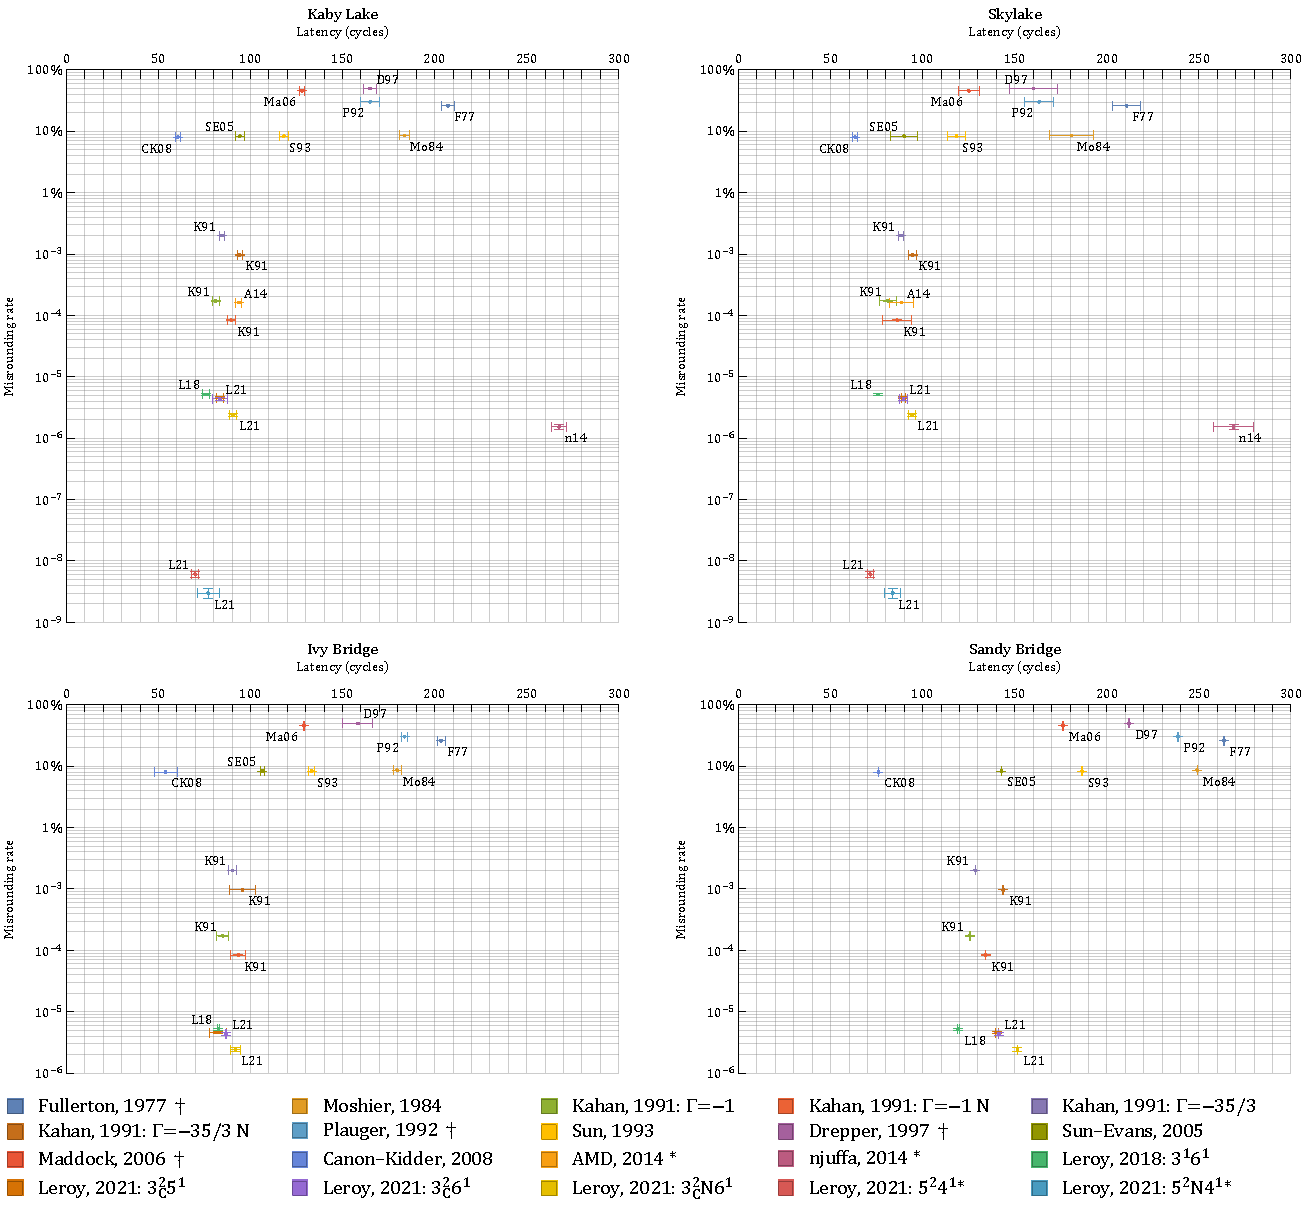
\includegraphics[width=\linewidth]{cbrt_latency_misrounding.pdf}
\caption{Latency of several implementations of the binary64 cube root, plotted against their misrounding rates, for various architectures.
The error bars are expanded uncertainties determined from the combined standard uncertainties and a coverage factor of $3$.
An asterisk marks methods that use FMA; an obelisk marks unfaithful methods.}
\end{adjustwidth}
\end{figure}

We consider the following method among our faithful ones, where the notation $p^qr^s$ means the generalized Lagny method of
degree $q$ and order $p$ is used in step~\ref{ThirdPrecision} and the generalized Lagny method of degree $r$ and order $s$
is used in step~\ref{HighOrder}, a subscript $\mathrm{C}$ indicates Canon optimization, the letter $\mathrm{N}$ indicates
the use of rounding to nearest in step~\ref{RoundedApproximation}, which otherwise uses directed rounding toward zero, and an
asterisk indicates the use of FMA as described in appendix~\ref{FMA}:
\begin{itemize}[nosep]
\item method $3^16^1$, used by Principia\footnote{The implementation in \#1802 uses a suboptimal evaluation strategy in step~\ref{ThirdPrecision}; the latencies shown are for the evaluation strategy described in appendix~\ref{Performance} instead.}
from pull request \href{https://github.com/mockingbirdnest/Principia/pull/1802}{\#1802},
in 2018, until it was replaced by a correctly-rounded method;
\item method $3^2_{\mathrm{C}}5^1$, which backs the correctly-rounded implementation without FMA;
\item method $3^2_{\mathrm{C}}6^1$ for comparison with $3^2_{\mathrm{C}}5^1$, see the discussion of step~\ref{HighOrder};
\item method $3^2_{\mathrm{C}}\mathrm{N}6^1$, the most accurate faithful method without FMA;
\item method $5^24^1*$, which backs the correctly-rounded implementation with FMA;
\item method $5^2\mathrm{N}4^1*$, the most accurate faithful method with FMA.
\end{itemize}
We compare these with following pre-existing implementations of the cube root:
\begin{itemize}[nosep]
\item W.~Fullerton's 1977 function DCBRT from FNLIB\footnote{We thank Peter Barfuss for translating this function from FORTRAN to
C++ for the purposes of this comparison.};
\item S.~L.~Moshier's 1984 function cbrt from the Cephes Mathematical Library;
\item W.~Kahan's 1991 methods described in \cite[3]{KahanBindel2001} ``to serve the IEEE Double precision and VAX G formats'',
implemented as written; Kahan recommends that the high-order step be of fourth order in that case, and gives two fourth
order methods; further, he does not specify how the rounding to a third of the precision should be performed,
so we end up with four possible implementations, identified by the coefficient of the asymptotic error,
$\mathrm Γ$ in Kahan's notation, and by the rounding direction of step~\ref{RoundedApproximation}
($\mathrm{N}$ for nearest, toward zero otherwise);
\item  P.~J.~Plauger's 1992 function cbrt from Dinkumware's C library, notably used by Microsoft's UCRT;
\item Sun Microsystems, Inc.'s 1993 function cbrt from the Freely Distributable LIBM;
\item U.~Drepper's 1997 function cbrt from the GNU C Library;
\item B.~Evans's 2005 modification of Sun's function cbrt, from the FreeBSD C library, also used by musl;
\item J.~Maddock's 2006 function boost::math::cbrt<double> from the Boost Library;
\item S.~Canon and J.~Kidder's 2008 function cbrt from Apple's Libm;
\item Advanced Micro Devices, Inc.'s 2014 function cbrt from libclc;
\item njuffa's 2014 function cbrt, given in a Stack Overflow answer to a question by P.~Cuoq about a correctly-rounded cube root.
\end{itemize}
The estimates of the latencies and their uncertainties were taken by supposing that the observed cycle counts follow
a three-parameter logarithmic normal distribution, with the latency of the benchmark loop being its terminus, the other two
parameters defining the distribution of random slowdowns. The maximum likelihood estimate of the terminus and the variance
of that estimate were computed as described in \cite{Cohen1951}.
The measured latency of a benchmark loop with a no-op function passed instead of the cube root was subtracted from these measurements,
with the standard uncertainties combined under the assumption that they were uncorrelated.

The misrounding rates were estimated by sampling a billion values uniformly at random from the set
$\intclop{1}{8}\Intersection\text{binary64}$
for methods with a misrounding rate greater than one per million, and a hundred billion values for the others.
The misrounding rates are given in table~\ref{TableMisroundingRates}.
\begin{table}[h!]
\setmainfont[Mapping=tex-text,
             Numbers={OldStyle, Monospaced},
             Ligatures={TeX, Common, Discretionary},
             SmallCapsFeatures={Letters=SmallCaps},
             Contextuals=WordFinal,]{Linux Libertine O}
\begin{center}
\begin{tabular}{rlr}
Method && Misrounding rate \\
\hline
Fullerton, 1977& $\dagger$  & $2.60500(14)\Multiply10^{-1}$ \\
Moshier, 1984&              & $8.55740(89)\Multiply10^{-2}$ \\
Kahan, 1991 & $\mathrm{Γ}=-1$        & $2.0044(15)\Multiply10^{-3}$  \\
\emph{ibid.}& $\mathrm{Γ}=-1$ $\mathrm{N}$     & $9.6466(99)\Multiply10^{-4}$  \\
\emph{ibid.}& $\mathrm{Γ}=-35/3$     & $1.7236(42)\Multiply10^{-4}$  \\
\emph{ibid.}& $\mathrm{Γ}=-35/3$ $\mathrm{N}$  & $8.367(29)\Multiply10^{-5}$   \\
Plauger, 1992& $\dagger$    & $3.02720(15)\Multiply10^{-1}$ \\
Sun,     1993&              & $8.31642(88)\Multiply10^{-2}$ \\
Drepper, 1997& $\dagger$    & $4.96271(16)\Multiply10^{-1}$ \\
Sun--Evans, 2005&           & $8.33311(88)\Multiply10^{-2}$ \\
Maddock, 2006& $\dagger$    & $4.56285(16)\Multiply10^{-1}$ \\
Canon--Kidder, 2008&        & $8.02588(86)\Multiply10^{-2}$ \\
AMD, 2014& $*$              & $1.6235(41)\Multiply10^{-4}$ \\
njuffa, 2014& $*$           & $1.529(40)\Multiply10^{-6}$ \\
Leroy, 2018 & $3^16^1$                        & $5.155(72)\Multiply10^{-6}$ \\
Leroy, 2021 & $3^2_{\mathrm{C}}5^1$           & $4.575(68)\Multiply10^{-6}$ \\
\emph{ibid.}& $3^2_{\mathrm{C}}6^1$           & $4.357(67)\Multiply10^{-6}$ \\
\emph{ibid.}& $3^2_{\mathrm{C}}\mathrm{N}6^1$ & $2.417(50)\Multiply10^{-6}$ \\
\emph{ibid.}& $5^24^1*$                       & $6.10(25)\Multiply10^{-9}$ \\
\emph{ibid.}& $5^2\mathrm{N}4^1*$             & $2.99(18)\Multiply10^{-9}$
\end{tabular}
\end{center}
\caption{Misrounding rates of various methods for the computation of a binary64 cube root.
An asterisk marks methods that use FMA; an obelisk marks unfaithful methods.\label{TableMisroundingRates}}
\end{table}

\emergencystretch 1em
\end{document}
